\chapter{MARTe Support Library}
\chaptermark{MARTe Support Library}


This chapter is about the core of the MARTe framework, i.e. the source code that let's GAMs work one with the other, reading data and write data from and to acquisition boards and take the control system in synch with all the plant system. This chapter address the dispatching of the different GAM's codes, the dispatching is done by the master thread that is bounded to the \texttt{RealTimeThread} object. No scheduling issues are addressed because there is no scheduling entity, the schedule of GAMs execution is done serially using a dependency analisys done a priori. \\


In this chapter we strongly analise sources in the \textit{MarteSupportLib} directory of the MARTe distribution package and then the MARTe executables coming with MARTe: \texttt{MARTe} and \texttt{MARTeService} (both in the root directory of the source package). \\


The chapter starts introducing a new type of component in the framework: the device driver (high level and low level device drivers). A real time framework to be deterministic must control each aspect of the control system, let's imagine that we have a real time algorithm that let's the feedback control waiting for input data from an acquisition board, if the device driver respond in microseconds but sometimes in milliseconds the responsiveness could not be sufficient for application we want, some delays can be caused from the Operating System so the developers of BaseLib/MARTe try to optimize and sometimes rewrite the device driver we use. \\



\section{IO Drivers}

This section addresses how device drivers are to be written to comply with the MARTe interface. First of all a device driver in MARTe is called a \textbf{Generic Acquisition Module} (\textit{GenericAcqModule} or \textit{GACQM}). A GACQM can be of different types regarding also the operating system on which is designed to work with. A common properties of all \textbf{Generic Acquisition Module}s is that once they start on a system they are never removed until MARTe has finished its execution and are permenently running (they have no ``run'' or ``start'' method); this characteristic make GACQM differ from GAM that are used within a precise slice of time calling the implemented control code once in a cycle. \\

\begin{figure}[h!]
 \begin{center}
  \includegraphics[width=0.78\textwidth]{MARTe/MARTe-GAcqM.eps}
  \caption{MARTe Generic Acquisitio Module}
  \label{f:MARTe:GAcqM}
 \end{center}
\end{figure}

Figure \ref{f:MARTe:GAcqM} is the UML diagram of the involved classes in this section, classes are just two: \texttt{TriggerTimeService} (quite usefull) and \texttt{GenericAcqModule} the most important class, every device driver in MARTe is a class that implements the \texttt{GenericAcqModule} interface.



\subsubsection{GenericAcqModule, TriggerTimeService}
\texttt{[GenericAcqModule.h, GenericAcqModule.cpp]} \\
The class \texttt{GenericAcqModule} is an abstract class (an interface with some methods implemented and with attributes) that abstracts a generic driver for an acquisition board. An acquisition board can generate data (synchronously or asynchcronously) and output data to the environment. But those are not the only tasks an acquisition board can do, a timing module, for example, can simply wake up an interrupt every predefined period or time instant. A \texttt{GenericAcqModule} abstracts all kind of external device that collect data, output data and generate events, i.e. also timing modules are \texttt{GenericAcqModule}. The end of an AD or DA conversion is also considered as an event. \\


A \texttt{GenericAcqModule} inherits from \texttt{GCNamedObject}, i.e. is garbage collectable and from \texttt{HttpInterface} (it can be ispected using an internet browser). The class relies on an internal defined class called \texttt{TriggerTimeService}. The class's interface follows. Such class is not necessary because it holds just one attribute \texttt{trigger} that points to a \texttt{TimeTriggeringServiceInterface} object. The class is only a sandbox that lets the user call in a safer way the \texttt{trigger} method of the holded class (via the \texttt{Trigger} method).

\begin{lstlisting}[
extendedchars=true,%
basicstyle=\fontfamily{pcr}\fontseries{m}\selectfont\footnotesize, %
stepnumber=1,%
numberstyle=\tiny,%
keywordstyle=\footnotesize\tt ,%
language=C++]
class TriggerTimeService{
private:
   TimeTriggeringServiceInterface* trigger;

public:
   TriggerTimeService();
   ~TriggerTimeService();

   bool Enable(TimeTriggeringServiceInterface* trigContext);
   bool Disable();
   void Trigger();
}
\end{lstlisting}

We switch now to analyse attributes of the \texttt{GenericaAcqModule} class.
The first attribute (\texttt{inputBoardInUse}) is a boolean, \texttt{True} if one \textit{GAM} is using this \texttt{GenericAcqModule} (\textit{GACQM}) as input, such decision restrict the usage of a GACQM from only one GAM at a time; \texttt{outputBoardInUse} is \texttt{True} if one GAM is using this module as output. \\


The attribute \texttt{numberOfInputChannels} is the umber of input channels in the module it's equal to the size of the data buffer (in \texttt{int32}); \texttt{numberOfOutputChannels} holds the number of output channels in the module. \\


Last group of attributes store informations regarding timing devices (or event generating boards); the array attribute \texttt{triggerService} lets the user register up to \texttt{MAX\_NUMBER\_OF\_TRIGGERING\_SERVICE} classes that will be informed (calling \texttt{Trigger} method) of the happening of an event; \texttt{nOfTriggeringServices} simply counts the number of registered \texttt{TriggerTimeService} objects.

\begin{lstlisting}[
extendedchars=true,%
basicstyle=\fontfamily{pcr}\fontseries{m}\selectfont\footnotesize, %
stepnumber=1,%
numberstyle=\tiny,%
keywordstyle=\footnotesize\tt ,%
language=C++]

protected:
   bool inputBoardInUse;
   bool outputBoardInUse;

   int32 numberOfInputChannels;
   int32 numberOfOutputChannels;

   TriggerTimeService triggerService[MAX_NUMBER_OF_TRIGGERING_SERVICE];
   int32 nOfTriggeringServices;
\end{lstlisting}

First two methods in the class are the constructor and the destructor. Then comes \texttt{ObjectLoadSetup}, \texttt{ObjectSaveSetup} and \texttt{ObjectDescription} that loads the setup from a CDB, save it on a CDB and output a  description of the object on a stream. \\


The method \texttt{IsSynchronizing} returns if the module is synchronizing, i.e. if it produces periodical events. the attribute \texttt{SetInputBoardInUse} set the input board in use, each module should use these method appropriately, for instance an ATM Module can only be used either as input module or output module; in this case both flags must be set by the \texttt{SetInputBoardInUse}/\texttt{SetOutputBordInUse} (the last follows) methods, for modules that can perform both input and output activities each flag should be set accordingly. \\

\paragraph{Input Boards}
The method \texttt{NumberOfInputs} returns the number of inputs to be read, \texttt{GetData} copies local input buffer in destination buffer, returns $0$ if data is not ready, below than $0$ if error, greater than $0$ if it all done.
The method \texttt{EnableAcquisition} enable the acquisition and is disabled by \texttt{DisableAcquisition} (is not really clear if it also disables the board or not). The method \texttt{StartSingleAcqusition} command the start of a single acquisition activity. \\

\paragraph{Output Boards}
The method \texttt{NumberOfOutputs} returns the number of outputs to be read, \texttt{WriteData} copies local data buffer in the board's buffer. \\

\paragraph{Timing Boards}
The method \texttt{EnableTimeService} enables and register a \texttt{TimeTriggeringServiceInterface} object (passed by argument to the method). \texttt{DisableTimeService} disables and deletes all registered \texttt{TimeTriggeringServiceInterface} objects. \texttt{Poll} is to be used by timing modules which support polling, no more explanations at this level are needed. \texttt{IsTimeModule} return \texttt{True} if the board is a Timing Device and it has the triggering service enabled.
\texttt{GetCTS}, \texttt{GetRTTN} and \texttt{GetUsecTime} are methods that returns the time in different forms. \\


For simulation purposes the method \texttt{PulseStart} was added. The method \texttt{NumberOfBuffers} returns the number of buffers used for acquisition; it is only used by boards with circular buffers and multiple acquisitions methods. \texttt{ProcessHttpMessage} is required by the \texttt{HttpInterface} and outputs an html page with information about the acquisition driver.

\begin{lstlisting}[
extendedchars=true,%
basicstyle=\fontfamily{pcr}\fontseries{m}\selectfont\footnotesize, %
stepnumber=1,%
numberstyle=\tiny,%
keywordstyle=\footnotesize\tt ,%
language=C++]
public:
   GenericAcqModule();
   virtual ~GenericAcqModule();

   virtual bool ObjectLoadSetup(ConfigurationDataBase& info,StreamInterface* err);
   virtual bool ObjectDescription(StreamInterface& s,bool full=False,
      StreamInterface* err=NULL)=0;

   virtual bool IsSynchronizing();
   virtual bool SetInputBoardInUse(bool on=True)=0;
   virtual bool SetOutputBoardInUse(bool on=True)=0;

   int32 NumberOfInputs() const;
   virtual int32 GetData(uint32 usecTime,int32* buffer,int32 bufferNumber=0)=0;

   virtual bool EnableAcquisition();
   virtual bool Poll();
   virtual bool DisableAcquisition();
   virtual bool StartSingleAcquisition();

   int32 NumberOfOutputs() const;
   virtual bool WriteData(uint32 usecTime,const int32* buffer)=0;

   bool EnableTimeService(TimeTriggeringServiceInterface* ts);
   bool DisableTimeService();
   bool IsTimeModule() const;

   virtual uint16 GetCTS();
   virtual uint32 GetRTTN();
   virtual int64 GetUsecTime();

   virtual bool PulseStart();

   virtual int32 NumberOfBuffers();
   virtual bool ProcessHttpMessage(HttpStream& hStream);
\end{lstlisting}



\subsection{Design Notes}
The class \texttt{TriggerTimeService} has only one attribute, by the way it can be deleted. Methods are not strictly necessary.



\section{Time Triggering Services}
This second section in this chapter will address time triggering services, such services associate temporal events with service routines; one temporal event can have many service routines associated with it. Temporal events can be the start or the end of an acquisition activity, a periodic clock, a timing sinchronization signal.. Temporal events can also generate other temporal events (think about a frequency divider). \\


In the past versions of MARTe there was only one type of \texttt{TimeTriggeringServiceInterface} and there is no interface defined, the class we are speaking about is the \texttt{ExternalTimeTriggeringService} class. Such functionalities are now played by the \texttt{InterruptDrivenTTS} class and the triggering activity on data polling is performed by the \texttt{DataPollingDrivenTTS} class (note that the synchronisation of the RealTimeThread is now done within the execution of the \texttt{TimeInputGAM}). \\

\begin{figure}[h!]
 \begin{center}
  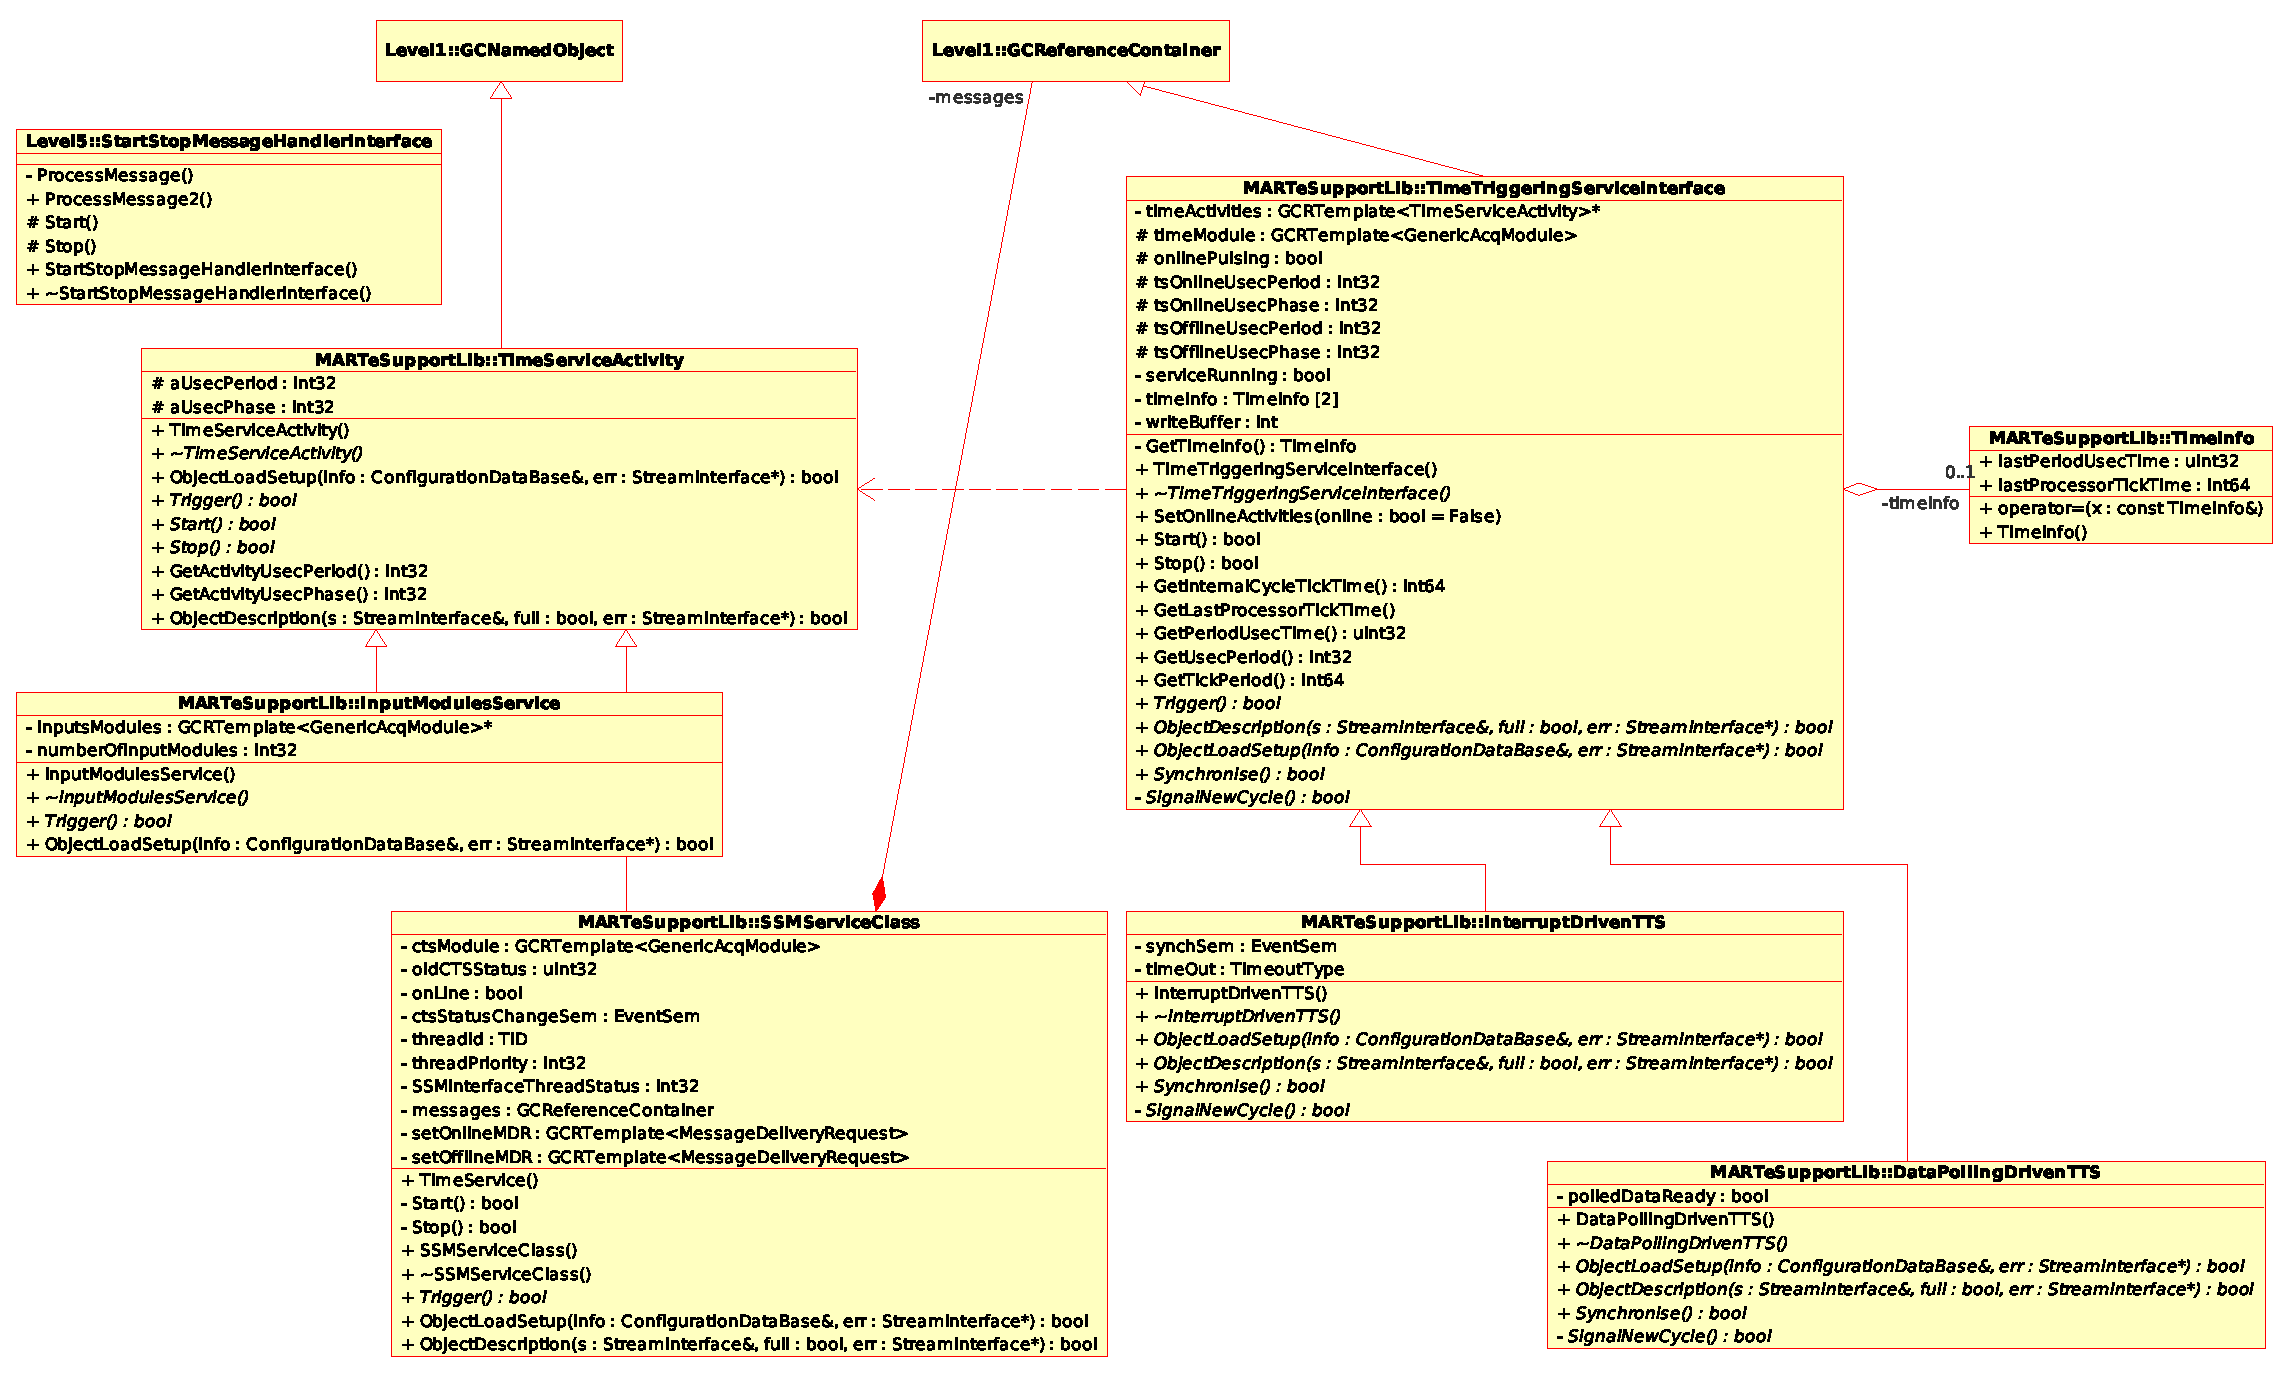
\includegraphics[width=\textwidth]{MARTe/MARTe-Timing.eps}
  \caption{MARTe Timing infrastructure}
  \label{f:MARTe:Timing}
 \end{center}
\end{figure}

In Figure \ref{f:MARTe:Timing} there is the UML schema depicting classes involved in this section. Such classes are:

\begin{itemize}
 \item TimeServiceActivity
 \item InputModulesService
 \item SSMServiceClass

 \item TimeTriggeringServiceInterface, TimeInfo
 \item InterruptDrivenTTS
 \item DataPollingDrivenTTS
\end{itemize}

In Figure \ref{f:MARTe:TimingClasses} is shown how classes interact and are linked one each other.

\begin{figure}[h!]
 \begin{center}
  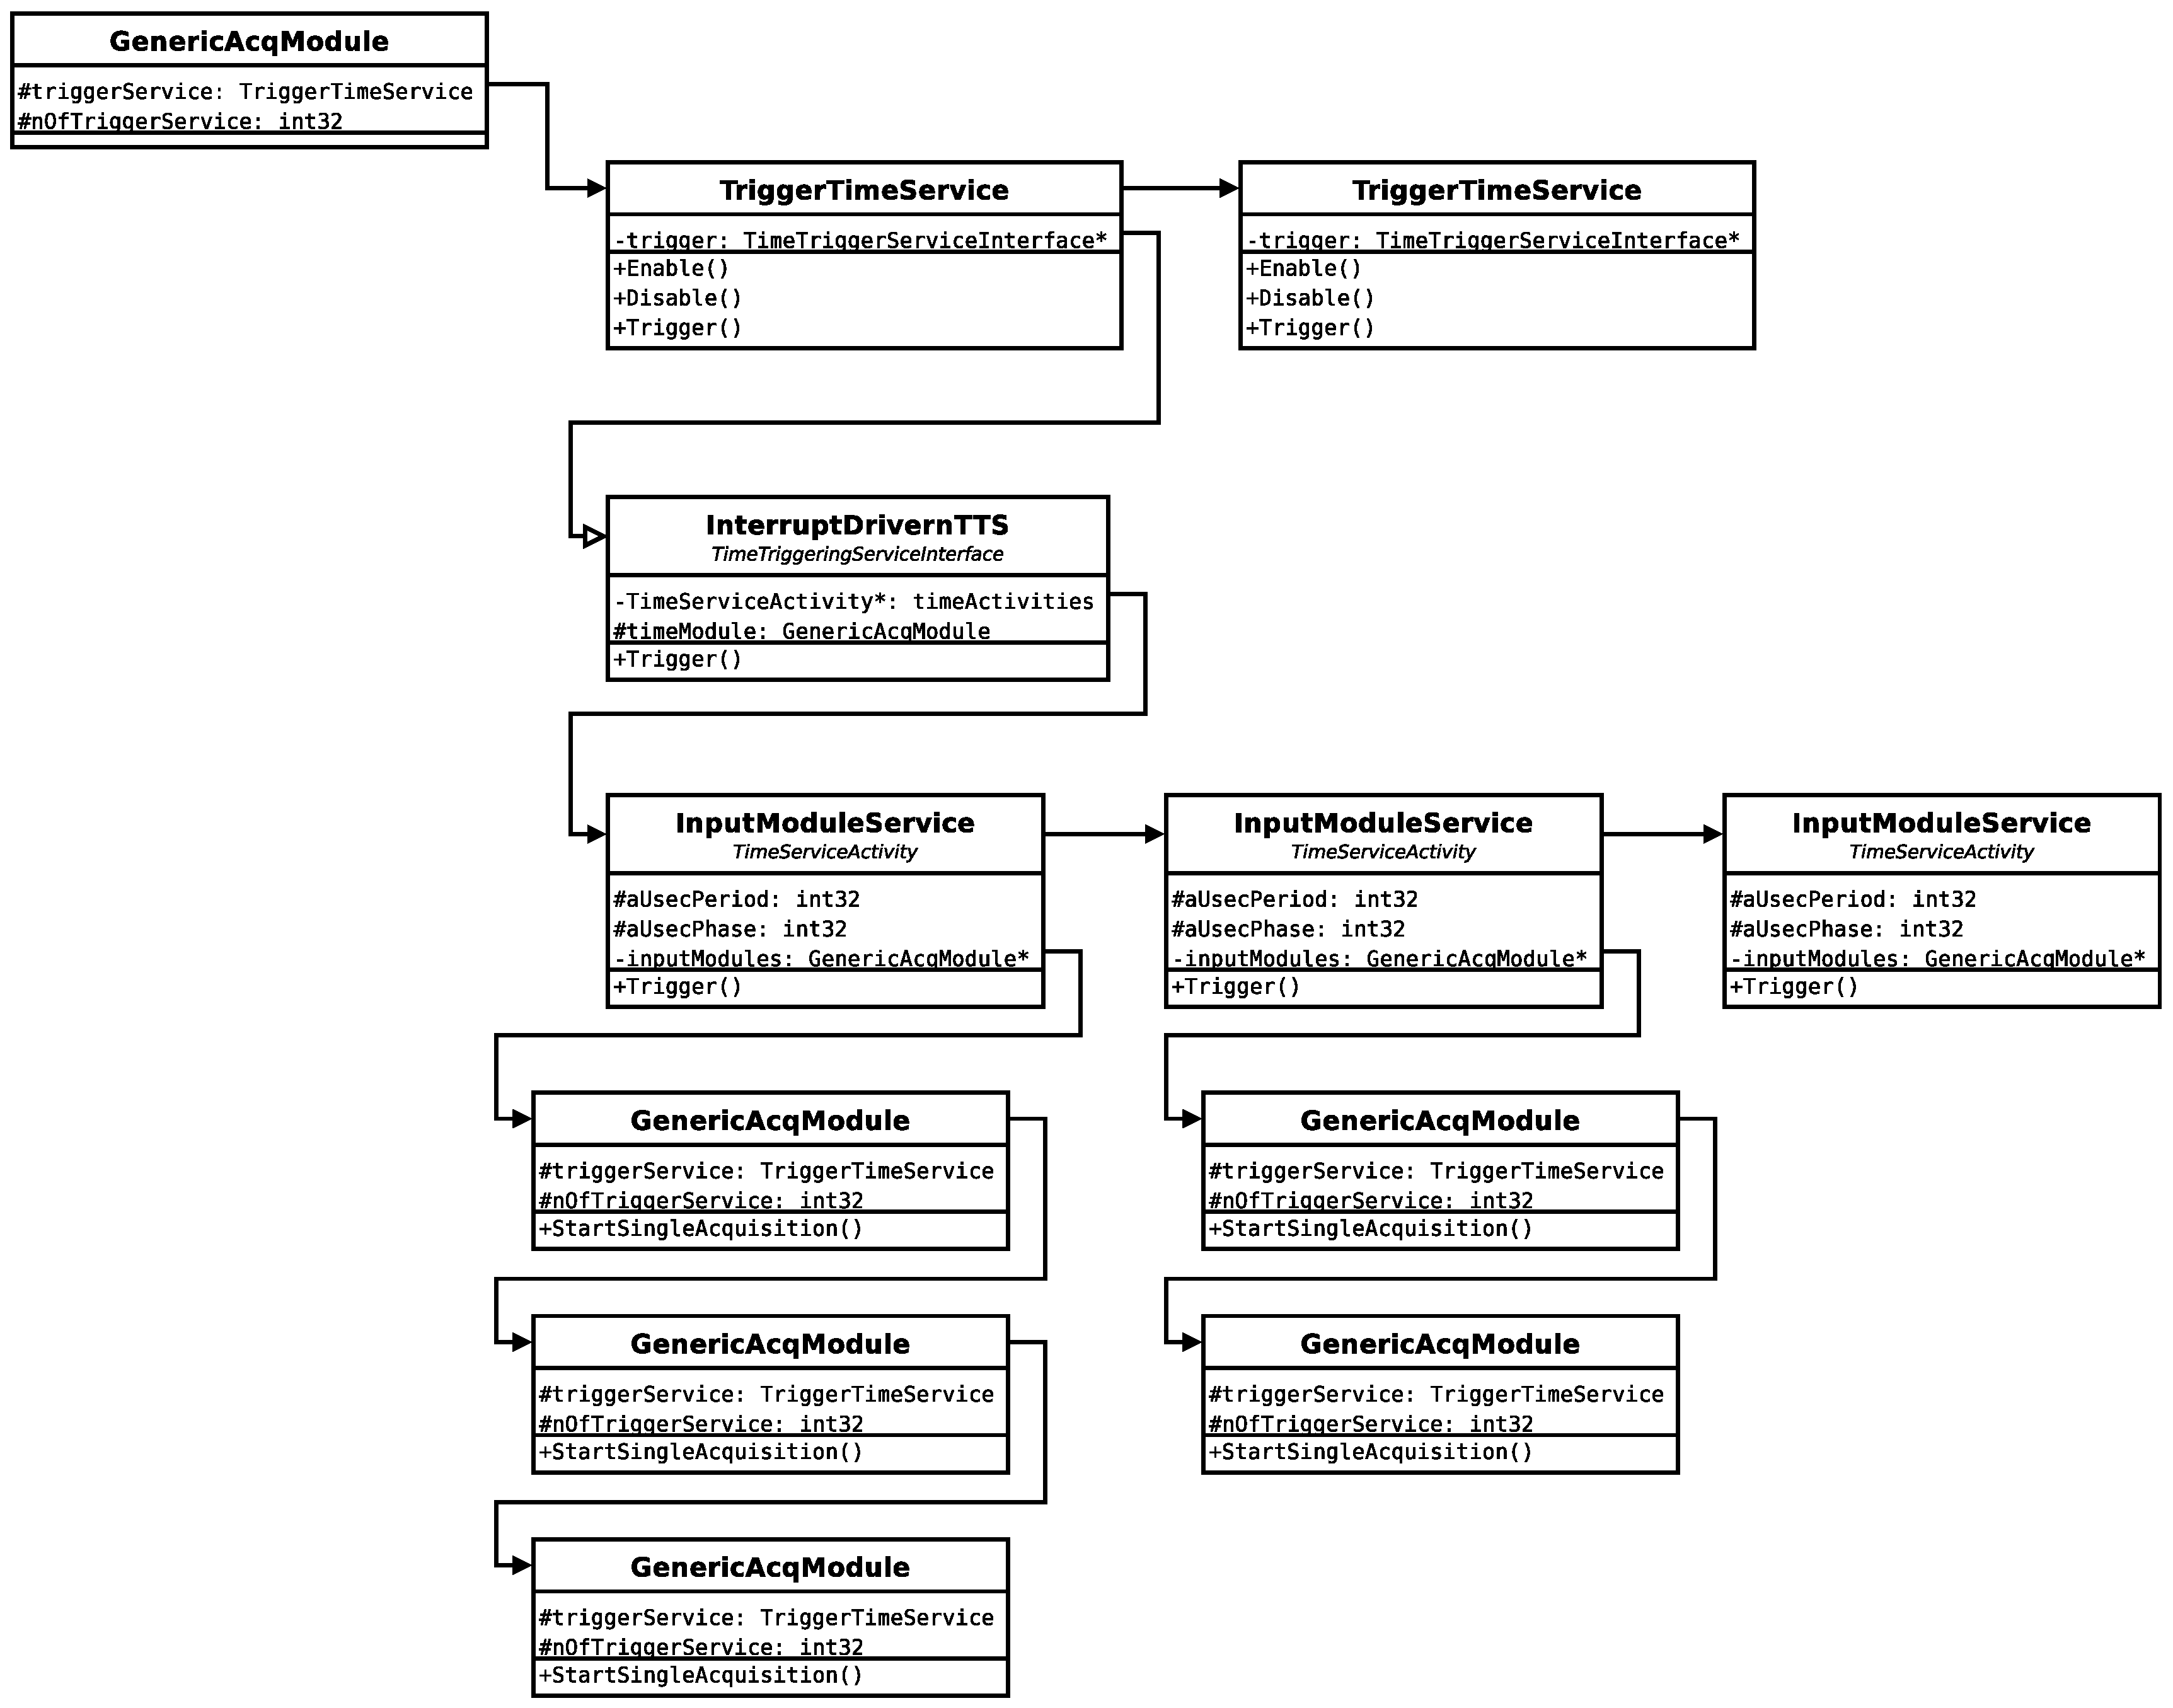
\includegraphics[width=0.83\textwidth]{MARTe/TimingClasses.eps}
  \caption{MARTe Timing Classes logical linkage}
  \label{f:MARTe:TimingClasses}
 \end{center}
\end{figure}



A GACQM can also be used to synchronise, in this case you need a \texttt{GAM} associated with the GACQM that calls its \texttt{Synchronize} method, the \texttt{InterruptDrivenTTS} offer a synchronization via ISR and semaphores but the \texttt{PollingDrivenTTS} offer a synchronization by polling a register (calling the Poll method of a synchronizing GACQM).



\subsubsection{TimeServiceActivity}
\texttt{[TimeServiceActivity.h, TimeServiceActivity.cpp]} \\
The class \texttt{TimeServiceActivity} abstract a periodic activity to do every \texttt{aUsecPeriod} with an \texttt{aUsecPhase} phase respect to a defined time event. Such class inherits only from \texttt{GCNamedObject}. There are only two attributes and we have just spend some words about them, the unit of time is the micro second.

\begin{lstlisting}[
extendedchars=true,%
basicstyle=\fontfamily{pcr}\fontseries{m}\selectfont\footnotesize, %
stepnumber=1,%
numberstyle=\tiny,%
keywordstyle=\footnotesize\tt ,%
language=C++]
protected:
   int32 aUsecPeriod;
   int32 aUsecPhase;
\end{lstlisting}

The constructor intializes the attributes to invalid values ($-1$), the destructor simply does nothing, \texttt{Trigger} isa pure virtual methotd, \texttt{Start} and \texttt{Stop} methods are the interface methods with the \texttt{StartStopMessageHandlerInterface} class and simply return true. The method \texttt{GetActivityUsecPeriod} returns the attribute \texttt{aUsecPeriod} and \texttt{GetActivityUsecPhase} returns \texttt{aUsecPhase}. \\


The method \texttt{ObjectLoadSetup} loads time service activity parameters from a CDB. \texttt{ObjectDescription} writes on a stream all module's parameters.

\begin{lstlisting}[
extendedchars=true,%
basicstyle=\fontfamily{pcr}\fontseries{m}\selectfont\footnotesize, %
stepnumber=1,%
numberstyle=\tiny,%
keywordstyle=\footnotesize\tt ,%
language=C++]
public:
   TimeServiceActivity();
   virtual ~TimeServiceActivity();

   virtual bool Trigger()=0;

   virtual bool Start();
   virtual bool Stop();

   inline int32 GetActivityUsecPeriod();
   inline int32 GetActivityUsecPhase();

   bool ObjectLoadSetup(ConfigurationDataBase& info,StreamInterface* err);
   bool ObjectDescription(StreamInterface& s,bool full=False,StreamInterface* err=NULL);
\end{lstlisting}



\subsubsection{InputModulesService}
\texttt{[InputModulesService.h, InputModulesService.cpp]} \\
The class \texttt{InputModulesService} is the first implementation of the class \texttt{TimeServiceActivity}. It holds a list of GACQM, on \textit{trigger}, at the correct period and phase, all GACQM's \texttt{StartSingleAcquisition} methods will be called. The attribute \texttt{inputsModules} is a pointer to an array of \texttt{GenericAcqModule}, \texttt{numberOfInputModules} count how many elements are in the array.

The constructor simply initialize the array that is populated via the \texttt{ObjectLoadSetup} and the distructor delete all elements in the array. The Trigger method call the \texttt{StartSingleAcquisition} method of each element in the array.

\begin{lstlisting}[
extendedchars=true,%
basicstyle=\fontfamily{pcr}\fontseries{m}\selectfont\footnotesize, %
stepnumber=1,%
numberstyle=\tiny,%
keywordstyle=\footnotesize\tt ,%
language=C++]
private:
   GCRTemplate<GenericAcqModule>* inputsModules;
   int32 numberOfInputModules;

public:
   InputModulesService();
   virtual ~InputModulesService();

   virtual bool Trigger();

   bool ObjectLoadSetup(ConfigurationDataBase& info,StreamInterface* err);
\end{lstlisting}



\subsubsection{SSMServiceClass}
\texttt{[SSMServiceClass.h, SSMServiceClass.cpp]} \\
The second implementation of the class \texttt{TimeServiceActivity} is the \texttt{SSMServiceClass}, i.e. the \textit{Supervisor State Machine Service Class}. \\


This is a dismissed class and can be taken only as an example, it will mimic the JET system supervisor state machine for MARTe receiving directly messages from the JET control (and timing) system; i.e. it was a replacement of part of the \textit{CODASLib}.\\


The first attribute, \texttt{ctsModule}, is a reference to the device driver module providing information about the pulse state, at JET the CTS is the \textit{Central Timing System}. The attribute \texttt{oldCTSStatus} is the previous state of the pulse; \texttt{onLine} tell us whether the pulse is in progress or not; \texttt{ctsStatusChangeSem} is a semaphore used to signal the change in the state of the pulse; \texttt{threadId} is a the identifier of the messaging handling task whos priority is setted with \texttt{threadPriority}; \texttt{SSMInterfaceThreadStatus} is the status of the task handling the messaging during pulse, related events: \textit{ACTIVE} or \textit{STOPPED}. \\


The attribute \texttt{messages} is a container of the messages for the \textit{State Machine} and \texttt{Real Time Thread}s; \texttt{setOnlineMDR} and \texttt{setOfflineMDR} are two message sender for the \textit{ONLINE} and \textit{OFFLINE} states.

\begin{lstlisting}[
extendedchars=true,%
basicstyle=\fontfamily{pcr}\fontseries{m}\selectfont\footnotesize, %
stepnumber=1,%
numberstyle=\tiny,%
keywordstyle=\footnotesize\tt ,%
language=C++]
private:
   GCRTemplate<GenericAcqModule> ctsModule;

   uint32 oldCTSStatus;

   bool onLine;

   EventSem ctsStatusChangeSem;
   TID threadId;
   int32 threadPriority;
   int32 SSMInterfaceThreadStatus;

   GCReferenceContainer messages;
   GCRTemplate <MessageDeliveryRequest> setOnlineMDR;
   GCRTemplate <MessageDeliveryRequest> setOfflineMDR;
\end{lstlisting}

The method \texttt{TimeService} is the messaging handling method; \texttt{Start} and \texttt{Stop} implements the \texttt{StartStopMessageHandlingInterface} starting and stopping the task handling pulse status change. \texttt{Trigger} is the method called by \texttt{TimeTriggeringServiceInterface}, note that the code in this method is executed only if $((ActualTime \% Period) == Phase)$.

\begin{lstlisting}[
extendedchars=true,%
basicstyle=\fontfamily{pcr}\fontseries{m}\selectfont\footnotesize, %
stepnumber=1,%
numberstyle=\tiny,%
keywordstyle=\footnotesize\tt ,%
language=C++]
   void TimeService();

   bool Start();
   bool Stop();

public:
   SSMServiceClass();
   virtual ~SSMServiceClass();

   virtual bool Trigger();

   bool ObjectLoadSetup(ConfigurationDataBase& info,StreamInterface* err);
   bool ObjectDescription(StreamInterface& s,bool full=False,StreamInterface* err=NULL);
\end{lstlisting}



\subsubsection{TimeTriggeringServiceInterface, TimeInfo}
\texttt{[TimeTriggeringServiceInterface.h, TimeTriggeringServiceInterface.cpp]} \\
The \texttt{TimeTriggeringServiceInterface} class is a container of \texttt{TimeServiceActivity} objects. The first attribute is infact a pointer to an array of \texttt{TimeServiceActivity} object (via the classic \texttt{GCRTemplate}).

The \texttt{TimeTriggeringServiceInterface} use the following \texttt{TimeInfo} structure. The structure holds a first attribute \texttt{lastPeriodUsecTime} that registered the last time obtained from the time module board (in $\mu$sec); next attribute, \texttt{lastProcessorTickTime}, is the last sample from the cpu internal clock as ticks. Then the \texttt{operator=} is overridden and also the constructor is redefined.

\begin{lstlisting}[
extendedchars=true,%
basicstyle=\fontfamily{pcr}\fontseries{m}\selectfont\footnotesize, %
stepnumber=1,%
numberstyle=\tiny,%
keywordstyle=\footnotesize\tt ,%
language=C++]
struct TimeInfo{
   uint32 lastPeriodUsecTime;
   int64 lastProcessorTickTime;

   inline void operator=(const TimeInfo &x);
   TimeInfo();
};
\end{lstlisting}

Now we switch speaking about the \texttt{TimeTriggeringServiceInterface} class that is a \texttt{GCReferenceContainer}.
The first attribute is a pointer to an array of \texttt{TimeServiceActivity} objects; \texttt{timeModule} is a reference to a \textit{TimeModule} (a timing board GACQM). \\


The attribute \texttt{onlinePulsing} is a flag to monitor online pulsing activities, to be controlled by the owning object; \texttt{tsOnlineUsecPeriod} is the time service period for online operations in $\mu$sec; \texttt{tsOnlineUsecPhase} is the time service phase for online operations in $\mu$sec; \texttt{tsOfflineUsecPeriod} is the time service period for offline operations in $\mu$sec; finally \texttt{tsOfflineUsecPhase} is the time service phase for offline operations in $\mu$sec. This design probably is thought not generally but designed for the JET control system. \\


The boolean attribute \texttt{serviceRunning} is a flag monitoring the status of the activities (\texttt{TimeServiceActivity}es). \texttt{timeInfo} is a double buffer containing the time information, there is always one write-only \texttt{TimeInfo} structure while the other is read-only; the \texttt{Trigger} method updates the index of the write-only buffer; such index is the attribute \texttt{writeBuffer}.

\begin{lstlisting}[
extendedchars=true,%
basicstyle=\fontfamily{pcr}\fontseries{m}\selectfont\footnotesize, %
stepnumber=1,%
numberstyle=\tiny,%
keywordstyle=\footnotesize\tt ,%
language=C++]
private:
   GCRTemplate<TimeServiceActivity>* timeActivities;

protected:
   GCRTemplate<GenericAcqModule> timeModule;

   bool onlinePulsing;
   int32 tsOnlineUsecPeriod;
   int32 tsOnlineUsecPhase;
   int32 tsOfflineUsecPeriod;
   int32 tsOfflineUsecPhase;

private:
   bool serviceRunning;
   TimeInfo timeInfo[2];
   int writeBuffer;
\end{lstlisting}

The method \texttt{GetTimeInfo} returns the read-only buffer (the last written timestamp buffer). The constructor initialize to zero all the attributes and the destructor simply calls all destructors. The method \texttt{SetOnlineActivities} set the attribute \texttt{onlinePulsing} to \texttt{online}; \texttt{Start} starts the \texttt{TimeTriggeringServiceInterface} and \texttt{Stop} stops it. \\


The method \texttt{GetInternalCycleTickTime} gets internal cycle time in ticks, asks to the \texttt{HRT} static class the current time in tick and subtract from that the \texttt{timeInfo.lastProcessorTickTime}; \texttt{GetLastProcessorTickTime} gets the last sample from the cpu internal clock as ticks; \texttt{GetPeriodUsecTime} gets time in $\mu$sec but as multiple of cycle time; \texttt{GetUsecPeriod} returns the period in $\mu$sec; \texttt{GetTickPeriod} returns the period in cpu ticks. \\


The method \texttt{Trigger} is to be called by a synchronising \texttt{GenericAcqModule} on data arrival; for data arrival that is signaled by interrupt, this method is to be called within the ISR; for data arrival that based on polling a register, this method is to be called within the \texttt{GetData} method of the synchronising \texttt{GenericAcqModule}. If $((ActualTime \% Period) == Phase)$ this method updates the \texttt{timeInfo} structure and calls the \texttt{SignalNewCycle} method, finally it checks if some activity is to be executed and if is the case calls its \texttt{Trigger} method. \\


The metohd \texttt{Synchronise} synchronizes the system to the cycle time, for triggering methods posted by interrupts the \texttt{Synchronise} waits on a semaphore to be posted by the ISR, namely the \texttt{SignalNewCycle} method; for triggering methods based on data arrival without interrupts, the \texttt{Synchronise} returns immediately  and the synchronisation is performed by the \texttt{GetData} method of the synchronising module. \\


The method \texttt{SignalNewCycle} is used within the \texttt{Trigger} method. It performs a set of activities marking the start of the new real-time cycle; for interrupt driven synchronising methods, the \texttt{SignalNewCycle} method posts the semaphore the \texttt{Synchronise} method is waiting on. For triggering methods based on data arrival, the SignalNewCycle returns without performing any activity.

\begin{lstlisting}[
extendedchars=true,%
basicstyle=\fontfamily{pcr}\fontseries{m}\selectfont\footnotesize, %
stepnumber=1,%
numberstyle=\tiny,%
keywordstyle=\footnotesize\tt ,%
language=C++]
private:
   inline TimeInfo GetTimeInfo() const;

public:
   TimeTriggeringServiceInterface();
   virtual ~TimeTriggeringServiceInterface();

   void SetOnlineActivities(bool online=False);
   bool Start();
   bool Stop();

   inline int64 GetInternalCycleTickTime() const;
   inline uint64 GetLastProcessorTickTime() const;
   inline uint32 GetPeriodUsecTime() const;
   inline int32 GetUsecPeriod() const;
   inline int64 GetTickPeriod() const;

   virtual bool Trigger();

   virtual bool ObjectDescription(StreamInterface& s,bool full=False,
      StreamInterface* err=NULL);
   virtual bool ObjectLoadSetup(ConfigurationDataBase& info,StreamInterface* err);

   virtual bool Synchronise()=0;

private:
   virtual bool SignalNewCycle()=0;
\end{lstlisting}



\subsubsection{InterruptDrivenTTS}
\texttt{[InterruptDrivenTTS.h, InterruptDrivenTTS.cpp]} \\
This is the first implementation of the \texttt{TimeTriggeringServiceInterface}, this implementation associate ad each interrupt a triggering event (i.e. an acquisition cycle). Interrupt can be generated from any type of board, acquisition board, network cards, timing modules etc.. \\


The attribute \texttt{synchSem} is an \texttt{EventSem} that will inform a task waiting on the \texttt{Synchronise} method (for example a \texttt{RealTimeThred}) that something is happening (the \texttt{Trigger} method is called); \texttt{timeOut} holds the semaphore timeout time.

The method \texttt{Synchronise} only waits on the \texttt{synchSem} and the method \texttt{SignalNewCycle} that is called by the \texttt{Trigger} method post the same semaphore.

\begin{lstlisting}[
extendedchars=true,%
basicstyle=\fontfamily{pcr}\fontseries{m}\selectfont\footnotesize, %
stepnumber=1,%
numberstyle=\tiny,%
keywordstyle=\footnotesize\tt ,%
language=C++]
private:
   EventSem synchSem;
   TimeoutType timeOut;

public:
   InterruptDrivenTTS();
   virtual ~InterruptDrivenTTS();

   virtual bool ObjectLoadSetup(ConfigurationDataBase& info,StreamInterface* err);
   virtual bool ObjectDescription(StreamInterface& s,bool full=False,
      StreamInterface* err=NULL);

   virtual bool Synchronise();

private:
   virtual bool SignalNewCycle();
\end{lstlisting}



\subsubsection{DataPollingDrivenTTS}
\texttt{[DataPollingDrivenTTS.h, DataPollingDrivenTTS.cpp]} \\
The class \texttt{DataPollingDrivenTTS} implements the \texttt{TimeTriggeringServiceInterface} in cases where we want to poll a registry for data arrival (for performance reasons) or we do not have a source of interrupts. 

The \texttt{DataPollingDrivenTTS} has only one boolean attribute \texttt{polledDataReady} that is true when data is ready. The method \texttt{Synchronise} synchronizes the system to the cycle time as expected, such method is implemented has a C loop testing the \texttt{GenericAcqModule::Poll} method return value, the synchronization is done by the \texttt{GetData} method in a \texttt{GenericAcqModule}. The method \texttt{SignalNewCycle} set \texttt{polledDataReady} to \texttt{True}, remember that is called by the \texttt{Trigger} method that is called by the \texttt{GetData} in the GACQM.

\begin{lstlisting}[
extendedchars=true,%
basicstyle=\fontfamily{pcr}\fontseries{m}\selectfont\footnotesize, %
stepnumber=1,%
numberstyle=\tiny,%
keywordstyle=\footnotesize\tt ,%
language=C++]
private:
   bool polledDataReady;

public:
   DataPollingDrivenTTS();
   ~DataPollingDrivenTTS()

   virtual bool ObjectLoadSetup(ConfigurationDataBase& info,StreamInterface* err);
   virtual bool ObjectDescription(StreamInterface& s,bool full=False,
      StreamInterface* err=NULL);

   virtual bool Synchronise();

private:
   virtual bool SignalNewCycle();
\end{lstlisting}



\subsection{Design Notes}
The first thing that is really noticing is that most objects in this section implements the \texttt{StartStopMessageHandlerInterface} but no one inherits from it; who has programmed those classes has forgot to declaring the inheritance relation probably. \\


Som words about the general purpose utilizability of the che class \texttt{TimeTriggeringServiceInterface} is generic enough? i.e. creating only two work cases: \textit{online} and \textit{offline} is enough for any existent plant system? Can exists any other states? States can be generally defined?

What happens if, using \texttt{DataPollingDrivenTTS}, no one call the \texttt{GetData} method? Probably the system will hang.. Differently if a polling module doesn't implement the \texttt{Poll} method all code continue to work without problems. \\


A modification that must be done is that when we call \texttt{GenericAcqModule::Trigger()} we have to pass by argument the associated event's time. In this way if, as usual in the code, one want to ask the event's time to the \texttt{TimeTriggeringServiceInterface} can do it but is not necessary so the code can be a bit more faster and simpler to read and understand. Now a \texttt{TimeTriggeringServiceInterface} must know how was calling it and asks to such GACQM the time. \\



\section{Execution Support}
Basically this section address all about execution of the real time control code. MARTe defines four realms or stages of code execution: the initialization, offline, online and safety. In each of this stages you can define your scheduling table, the schedulability entities are the GAMs (calling the \texttt{Execute} method). Who is in charge to dispatch the execution and choose (following a state machine) in which realm we are now executing is the \texttt{RealTimeThread}. To achieve bounded time responsiveness a single \texttt{RealTimeThread} should be executed to a single processor core without other threads, the scheduling of GAM's execution is done by a data dependency analisys offline. If a system can take advantage of many cores a control algorithm can also be parallelized (this feature is not supported right now). \\


In this section the \texttt{RealTimeThread} is presented and some other classes to register code performances are analised. Such performance data can be used to make schedulability analisys and also to try to understand which part of the code lack in performance. In Figure \ref{f:MARTe:Support} an UML class diagram showing the class relation between classes involved in this section is depicted, a list of classes follows. \\

\begin{figure}[h!]
 \begin{center}
  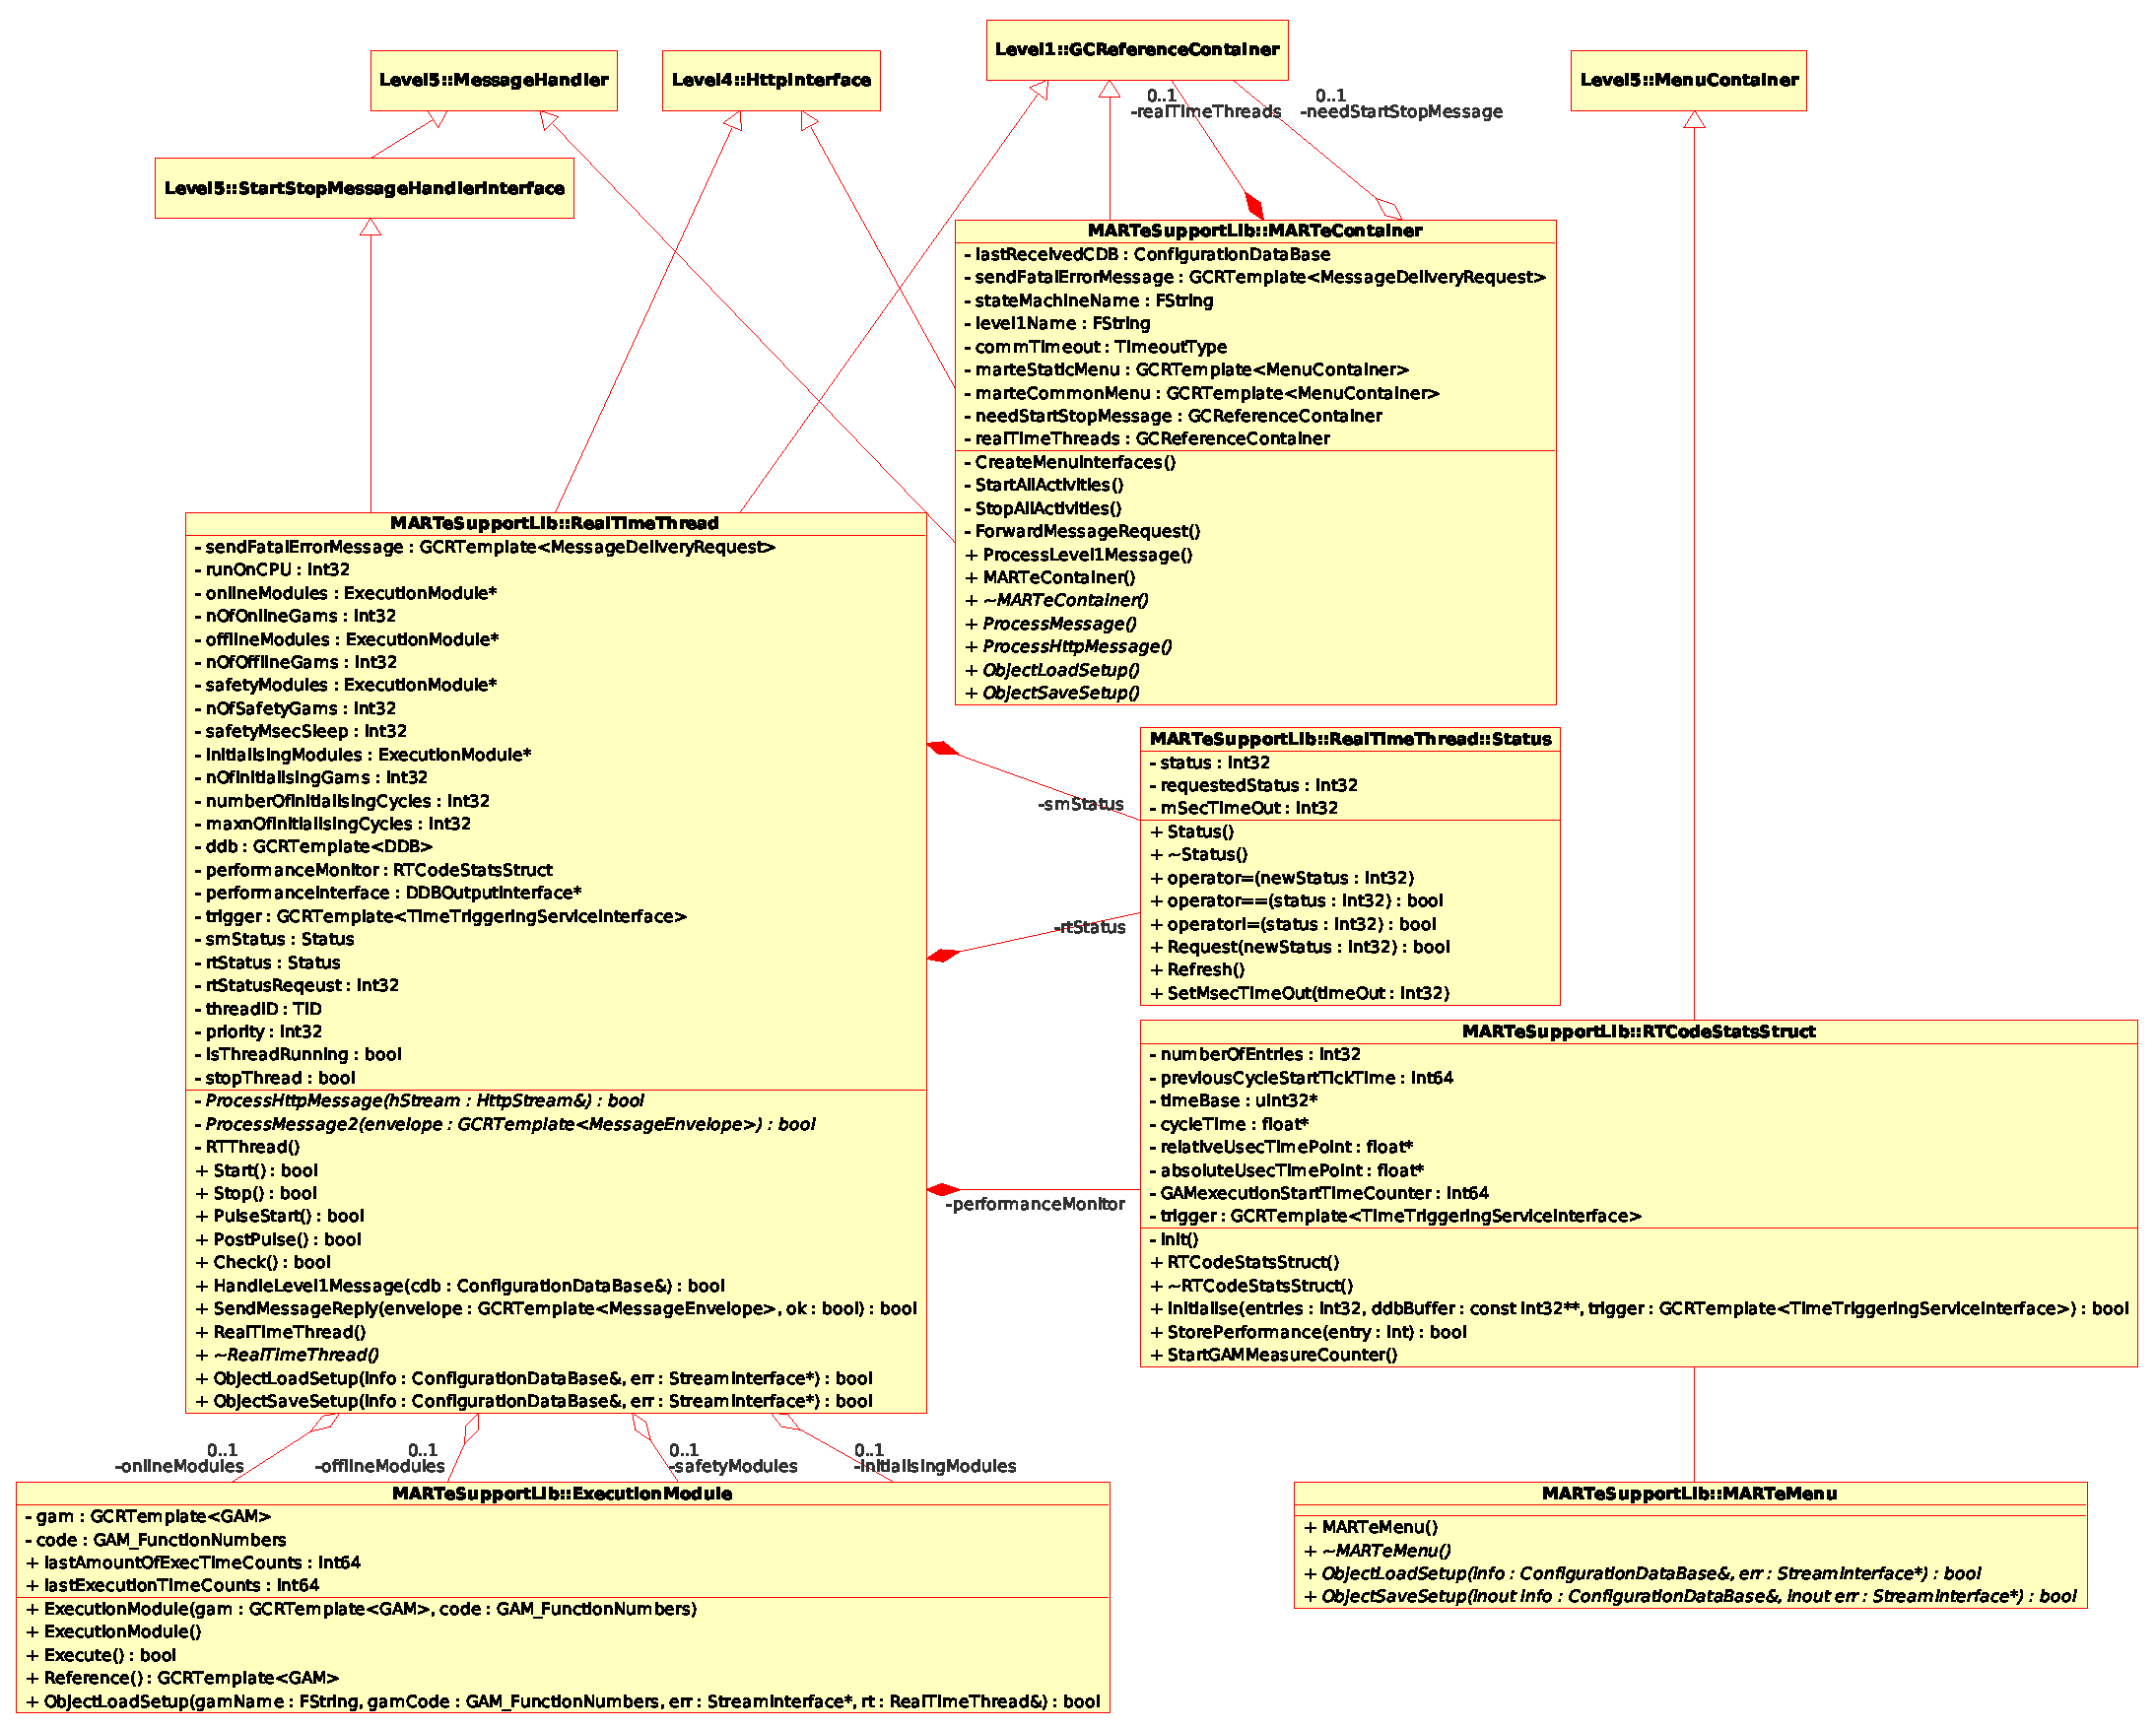
\includegraphics[width=\textwidth]{MARTe/MARTe-Support.eps}
  \caption{MARTe Executor infrastructure (GAM's dispatcher)}
  \label{f:MARTe:Support}
 \end{center}
\end{figure}

\begin{itemize}
 \item RTCodeStatsStruct
 \item ExecutionModule
 \item RealTimeThread, Status
 \item MARTeMenu
 \item MARTeContainer
\end{itemize}


Let's spend some words to the last class \texttt{MARTeContainer}: it is MARTe. Well MARTe infact is a collection of a \texttt{ConfigurationDataBase}, a fatal error message dispatcher/receiver, an associated state machine, a level1 message receiver, a menu based interface and a set of \texttt{RealTimeThread}s. All this list is well depicted in Figure \ref{f:MARTe:MARTeContainer}.

Note that if a \texttt{MARTeContainer} has an associated state machine such machine is outside the \texttt{MARTeContainer} but for example \texttt{RealTimeThread}s are part of it. The border between what is inside and what is not isn't well defined and require a deep understanding of the whole project. \\

\begin{figure}[h!]
 \begin{center}
  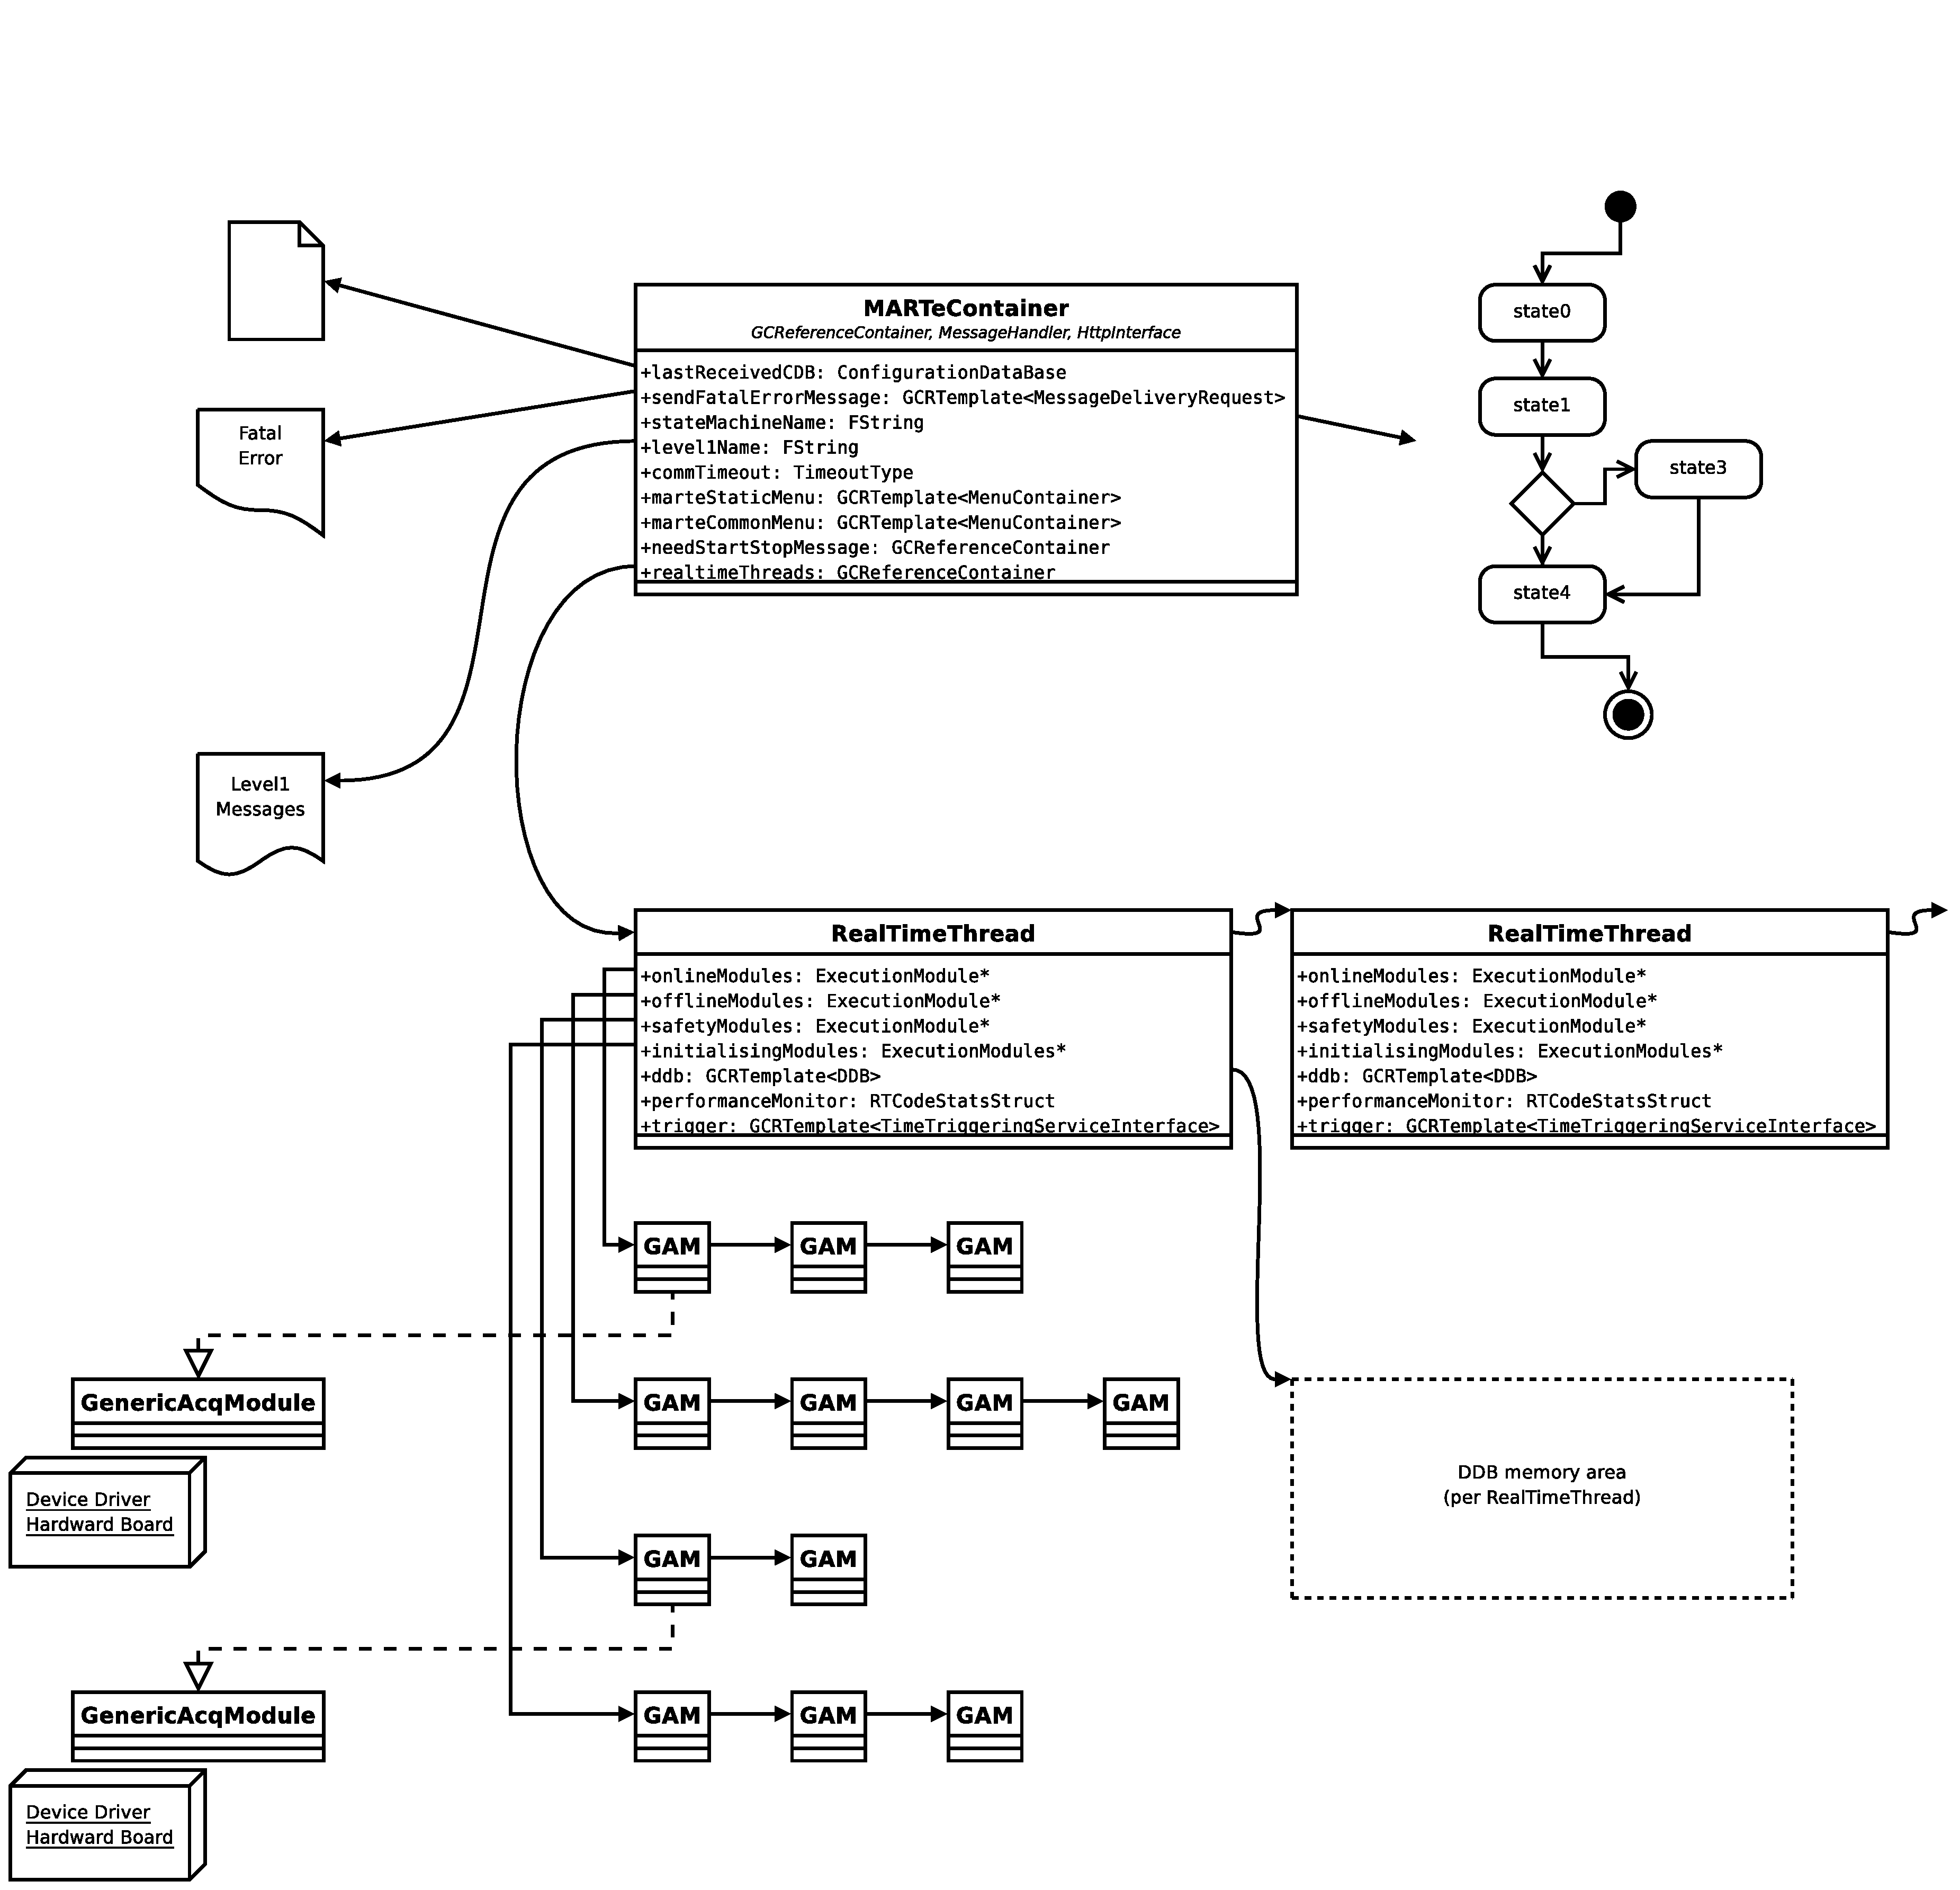
\includegraphics[width=\textwidth]{MARTe/MARTeContainer.eps}
  \caption{MARTe Container UML/logical scheme}
  \label{f:MARTe:MARTeContainer}
 \end{center}
\end{figure}
\clearpage



\subsection{RTCodeStatsStruct}
\texttt{[RTCodeStatsStruct.h]} \\
The class \texttt{RTCodeStatsStruct} is the Real-Time code performance monitor, i.e. it monitors the execution time of the code. Then we will see how it is used inside the \texttt{RealTimeThread} entity. \\


The time information collected are stored in a DDB memory area, it is not compulsory to store them in a DDB memory area, the \texttt{RTCodeStatsStruct} class require an \texttt{int32*} as the address where to store the statistics. In Figure \ref{f:MARTe:StatsStruct} is illustrated the format of the time data that will be stored (the number of the saved entry must be precalcolated).

\begin{figure}[h!]
 \begin{center}
  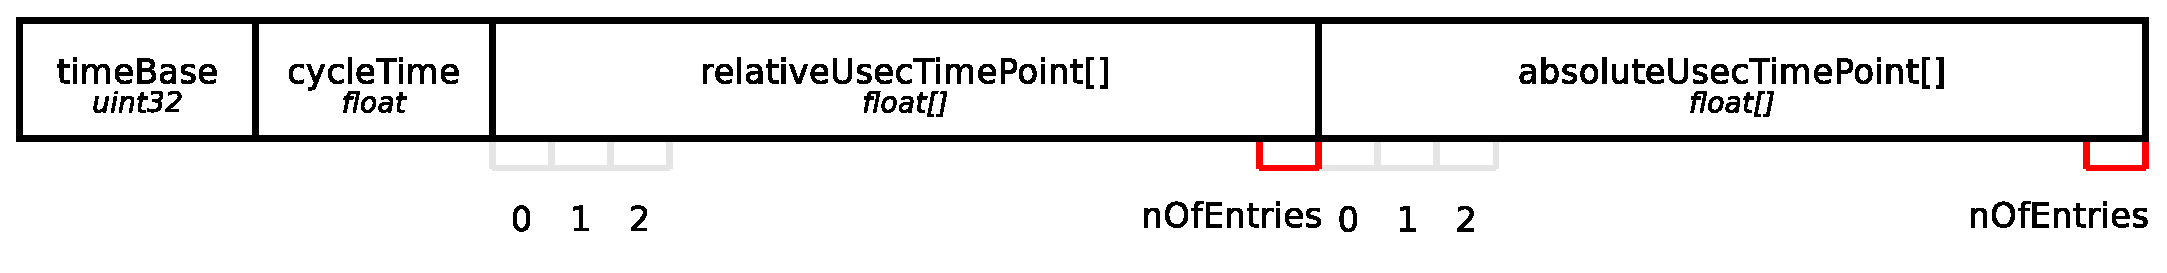
\includegraphics[width=0.92\textwidth]{MARTe/StatsStruct.eps}
  \caption{Format of the StatsStruct in the DDB memory area}
  \label{f:MARTe:StatsStruct}
 \end{center}
\end{figure}

The number of entries to monitor are saved in the \texttt{numberOfEntries} attribute. The pointers to the DDB memory area are \texttt{timeBase}, \texttt{cycleTime}, \texttt{relativeUsecTimePoint} and \texttt{absoluteUsecTimePoint} (those attributes are just depicted in Figure \ref{f:MARTe:StatsStruct}).

The attribute \texttt{previousCycleStartTickTime} holds the previous start of cycle time, \texttt{GAMexecutionStartTimeCounter} saves the execution start time for this module (see method \texttt{StartGAMMeasureCounter}). The attribute \texttt{trigger} is a reference to the external time or triggering service of associated to the \texttt{RealTimeThread}; methods \texttt{GetInternalCycleTickTime}, \texttt{GetLastProcessorTickTime} and \texttt{GetPeriodUsecTime} of the \texttt{TimeTriggeringServiceInterface} class are used.

\begin{lstlisting}[
extendedchars=true,%
basicstyle=\fontfamily{pcr}\fontseries{m}\selectfont\footnotesize, %
stepnumber=1,%
numberstyle=\tiny,%
keywordstyle=\footnotesize\tt ,%
language=C++]
private:
   int32 numberOfEntries;

   int64 previousCycleStartTickTime;
   int64 GAMexecutionStartTimeCounter;

   uint32* timeBase;
   float* cycleTime;
   float* relativeUsecTimePoint;
   float* absoluteUsecTimePoint;

   GCRTemplate<TimeTriggeringServiceInterface> trigger;
\end{lstlisting}

The method \texttt{Init} initialise all attributes for construction to zero or \texttt{NULL}. \texttt{Initialise} initialises the \texttt{RTCodeStatsStruct} attributes using the parameters passed by; such method must be called in the \textit{PRE PULSE} state, because during the loading of the library and objects DDB buffers are not available yet. Like in Figure \ref{f:MARTe:StatsStruct} the code assumes that the first entry in the DDB data buffer is the time in microseconds relative to the monitoring measurement, the cycle time is the following entry, followed by the relative time points and the absolute time points. \\

The method \texttt{StorePerformance} computes performance for entry \texttt{entry}, i.e. must be called at the end of the execution of the entry-n GAM. \texttt{StartGAMMeasureCounter} signals a new performance measurament cycle.

\begin{lstlisting}[
extendedchars=true,%
basicstyle=\fontfamily{pcr}\fontseries{m}\selectfont\footnotesize, %
stepnumber=1,%
numberstyle=\tiny,%
keywordstyle=\footnotesize\tt ,%
language=C++]
   void Init();
public:
   RTCodeStatsStruct();
   ~RTCodeStatsStruct();

   bool Initialise(int32 entries,const int32* ddbBuffer,
       GCRTemplate<TimeTriggeringServiceInterface> trigger);

   bool StorePerformance(int entry);
   void StartGAMMeasureCounter();
\end{lstlisting}



\subsection{ExecutionModule}
\texttt{[RealTimeThread.h, RealTimeThread.cpp]} \\
The \texttt{ExecutionModule} class is a wrapper class that lets you call the \texttt{Execute} method of a GAM without specifing the \texttt{GAM\_FunctionNumber} because is just embedded in the \texttt{ExecutionModule}, such class contain also a the instance of the \texttt{GAM} required.

The \texttt{Execute} method also measure the time consumed by the execution of the \texttt{GAM::Execute} method each time is called. The time is measured using the \texttt{BaseLib::Level0::HRT} class and is stored in the public attribute \texttt{lastAmountOfExecTimeCounts}.

\begin{lstlisting}[
extendedchars=true,%
basicstyle=\fontfamily{pcr}\fontseries{m}\selectfont\footnotesize, %
stepnumber=1,%
numberstyle=\tiny,%
keywordstyle=\footnotesize\tt ,%
language=C++]
private:
   GCRTemplate<GAM> gam;
   GAM_FunctionNumbers code;

public:
   int64 lastAmountOfExecTimeCounts;
   int64 lastExecutionTimeCounts;

   ExecutionModule(GCRTemplate<GAM> gam,GAM_FunctionNumbers code);
   ExecutionModule();

   bool Execute();

   GCRTemplate<GAM> Reference();
   bool ObjectLoadSetup(FString gamName, GAM_FunctionNumbers gamCode,
      StreamInterface* err, RealTimeThread& rt);
\end{lstlisting}



\subsection{RealTimeThread, Status}
\texttt{[RealTimeThread.h, RealTimeThread.cpp]} \\
Before introducing the most important class of MARTe we need to spend some words on its internal class \texttt{Status} whos interface follow in the text. Such internal class lets the \texttt{RealTimeThread} have a personal/private developed state machine that has no link to the one you can find in BaseLib (this could be a limitation for the general utilizability/applicability of MARTe). \\


The class \texttt{Status} has the attribute \texttt{status} that holds one of differents values  that represent the state itself. \\


The attribute \texttt{requestedStatus} holds one of the previous values and is the required next state to move; \texttt{mSecTimeOut} is the timeout for the request to be completed. Some operator are redefined to ease the copy and compare of many \texttt{Status} classes. \\


The method \texttt{Request} requests a change in the status and waits by sleeping one millisecond by one millisecond for the accomplishment. \texttt{Refresh} copies the requested status on the \texttt{status} attribute. \texttt{SetMsecTimeOut} sets the timeout value.

\begin{lstlisting}[
extendedchars=true,%
basicstyle=\fontfamily{pcr}\fontseries{m}\selectfont\footnotesize, %
stepnumber=1,%
numberstyle=\tiny,%
keywordstyle=\footnotesize\tt ,%
language=C++]
class Status{
private:
   int32 status;
   int32 requestedStatus;
   int32 mSecTimeOut;

public:
   Status();
   ~Status();

   Status& operator=(int32 newStatus);
   bool operator == (int32 status)
   bool operator != (int32 status);

   bool Request(int32 newStatus);
   void Refresh();
   void SetMsecTimeOut(int32 timeOut);
};
\end{lstlisting}


% ----------------------------------------------------------------------------- %
% ----------------------------------------------------------------------------- %
% ----------------------------------------------------------------------------- %


We go over analising the \texttt{RealTimeThread} class that's the class representing a real time thread of execution, it inherits from \texttt{GCReferenceContainer}, and implements the \texttt{StartStopMessageHandlerInterface} and \texttt{HttpInterface} interfaces. \\


The first attribute is \texttt{sendFatalErrorMessage} a \texttt{MessageDeliveryRequest} object that enables the real-time thread send fatal error messages. The attribute \texttt{trigger} is a \texttt{TimeTriggeringServiceInterface} that lets the real-time thread synchronizing on some external events (one \texttt{RealTimeThread} has only one \texttt{TimeTriggeringServiceInterface} associated with it
). \\


The attribute \texttt{smStatus} is the \textit{State Machine Status} a state machine changing its state by message processing (i.e. it receives messages from the plant state machine and then convert it in internal BaseLib messages). Possible values of this state are (declared at the top of the cpp):
\begin{lstlisting}[
extendedchars=true,%
basicstyle=\fontfamily{pcr}\fontseries{m}\selectfont\footnotesize, %
stepnumber=1,%
numberstyle=\tiny,%
keywordstyle=\footnotesize\tt ,%
language=C++]
static const int32 SM_IDLE         = 101;
static const int32 SM_WAITING_PRE  = 102;
static const int32 SM_PREPULSE     = 103;
static const int32 SM_PULSING      = 104;
static const int32 SM_POSTPULSE    = 105;
static const int32 SM_INITIALISING = 106;
\end{lstlisting}

In the \texttt{SM\_IDLE} it performs offline activities, in \texttt{SM\_WAITING\_PRE} it performs the \texttt{PulseStart} activities (method) before switching to \texttt{SM\_PULSING}, in \texttt{SM\_PULSING} it performs online activities, in \texttt{SM\_POSTPULSE} it performs the \texttt{PostPulse} activities before switching to \texttt{SM\_IDLE}, as we will see in Figure \ref{f:MARTe:RealTimeThread:StateMachine} is not really like that, there are some problems in the design of those combined state machines. The other state machine is implemented as the attribute \texttt{rtStatus} and is the status of the \texttt{RealTimeThread} object. Values are:

\begin{lstlisting}[
extendedchars=true,%
basicstyle=\fontfamily{pcr}\fontseries{m}\selectfont\footnotesize, %
stepnumber=1,%
numberstyle=\tiny,%
keywordstyle=\footnotesize\tt ,%
language=C++]
/// UNDEFINED STATE - RTApplicationThread has not been initialized
static const int32 RTAPP_UNDEFINED = 0xFFFFFFFF;
/// READY STATE - RTApplicationThread object has been initialised
static const int32 RTAPP_READY     = 0x00000000;
/// SAFETY STATE - When a major fault has been identified
static const int32 RTAPP_SAFETY    = 0x00000002;
\end{lstlisting}

The attribute \texttt{rtStatusRequest} switch status request. It is used to avoid the presence of the mutex semaphore into the real-time thread. The method that requires the change asks for the transition to the \texttt{RTAPP\_UNDEFINED} and waits that \texttt{rtStatus} assumes the requested value. \\


Now comes \textbf{four} sets of vectors of GAMs that will be executed in differents combined states of the \texttt{RealTimeThread} and the plant state machine, Figure \ref{f:MARTe:RealTimeThread:StateMachine} is a schema with some of the messages transition between combined states.

The attribute \texttt{onlineModules} is a vector of execution modules for real time activities, the number of gams in the online activities vector is \texttt{nOfOnlineGams}.

The attribute \texttt{offlineModules} is a vector of execution modules for the offline activities, the number of gams in the onffline activities vector is \texttt{nOfOfflineGams}.

The attribute \texttt{safetyModules} is a vector of execution modules for safety activities, the number of gams in the safety activities vector is \texttt{nOfSafetyGams}; \texttt{safetyMsecSleep} is the millisecond sleep time if not module is specified in the \texttt{nOfSafetyGams} vector.

The attribute \texttt{initialisingModules} is a vector of execution modules that need an initialisation phase, the number of gams in the initialisation activities vector is \texttt{nOfInitialisingGams}; \texttt{numberOfInitialisingCycles} is the number of consecutive initialising cycles and \texttt{maxnOfInitialisingCycles} is the maximum number of initialising cycles. \\

\begin{lstlisting}[
extendedchars=true,%
basicstyle=\fontfamily{pcr}\fontseries{m}\selectfont\footnotesize, %
stepnumber=1,%
numberstyle=\tiny,%
keywordstyle=\footnotesize\tt ,%
language=C++]
   GCRTemplate <MessageDeliveryRequest> sendFatalErrorMessage;

   GCRTemplate<TimeTriggeringServiceInterface> trigger;

   Status smStatus;
   Status rtStatus;
   int32 rtStatusRequest;

   ExecutionModule* onlineModules;
   int32 nOfOnlineGams;

   ExecutionModule* offlineModules;
   int32 nOfOfflineGams;

   ExecutionModule* safetyModules;
   int32 nOfSafetyGams;
   int32 safetyMsecSleep;

   ExecutionModule* initialisingModules;
   int32 nOfInitialisingGams;
   int32 numberOfInitialisingCycles;
   int32 maxnOfInitialisingCycles;
\end{lstlisting}



\begin{sidewaysfigure}[h!]
 \centering
 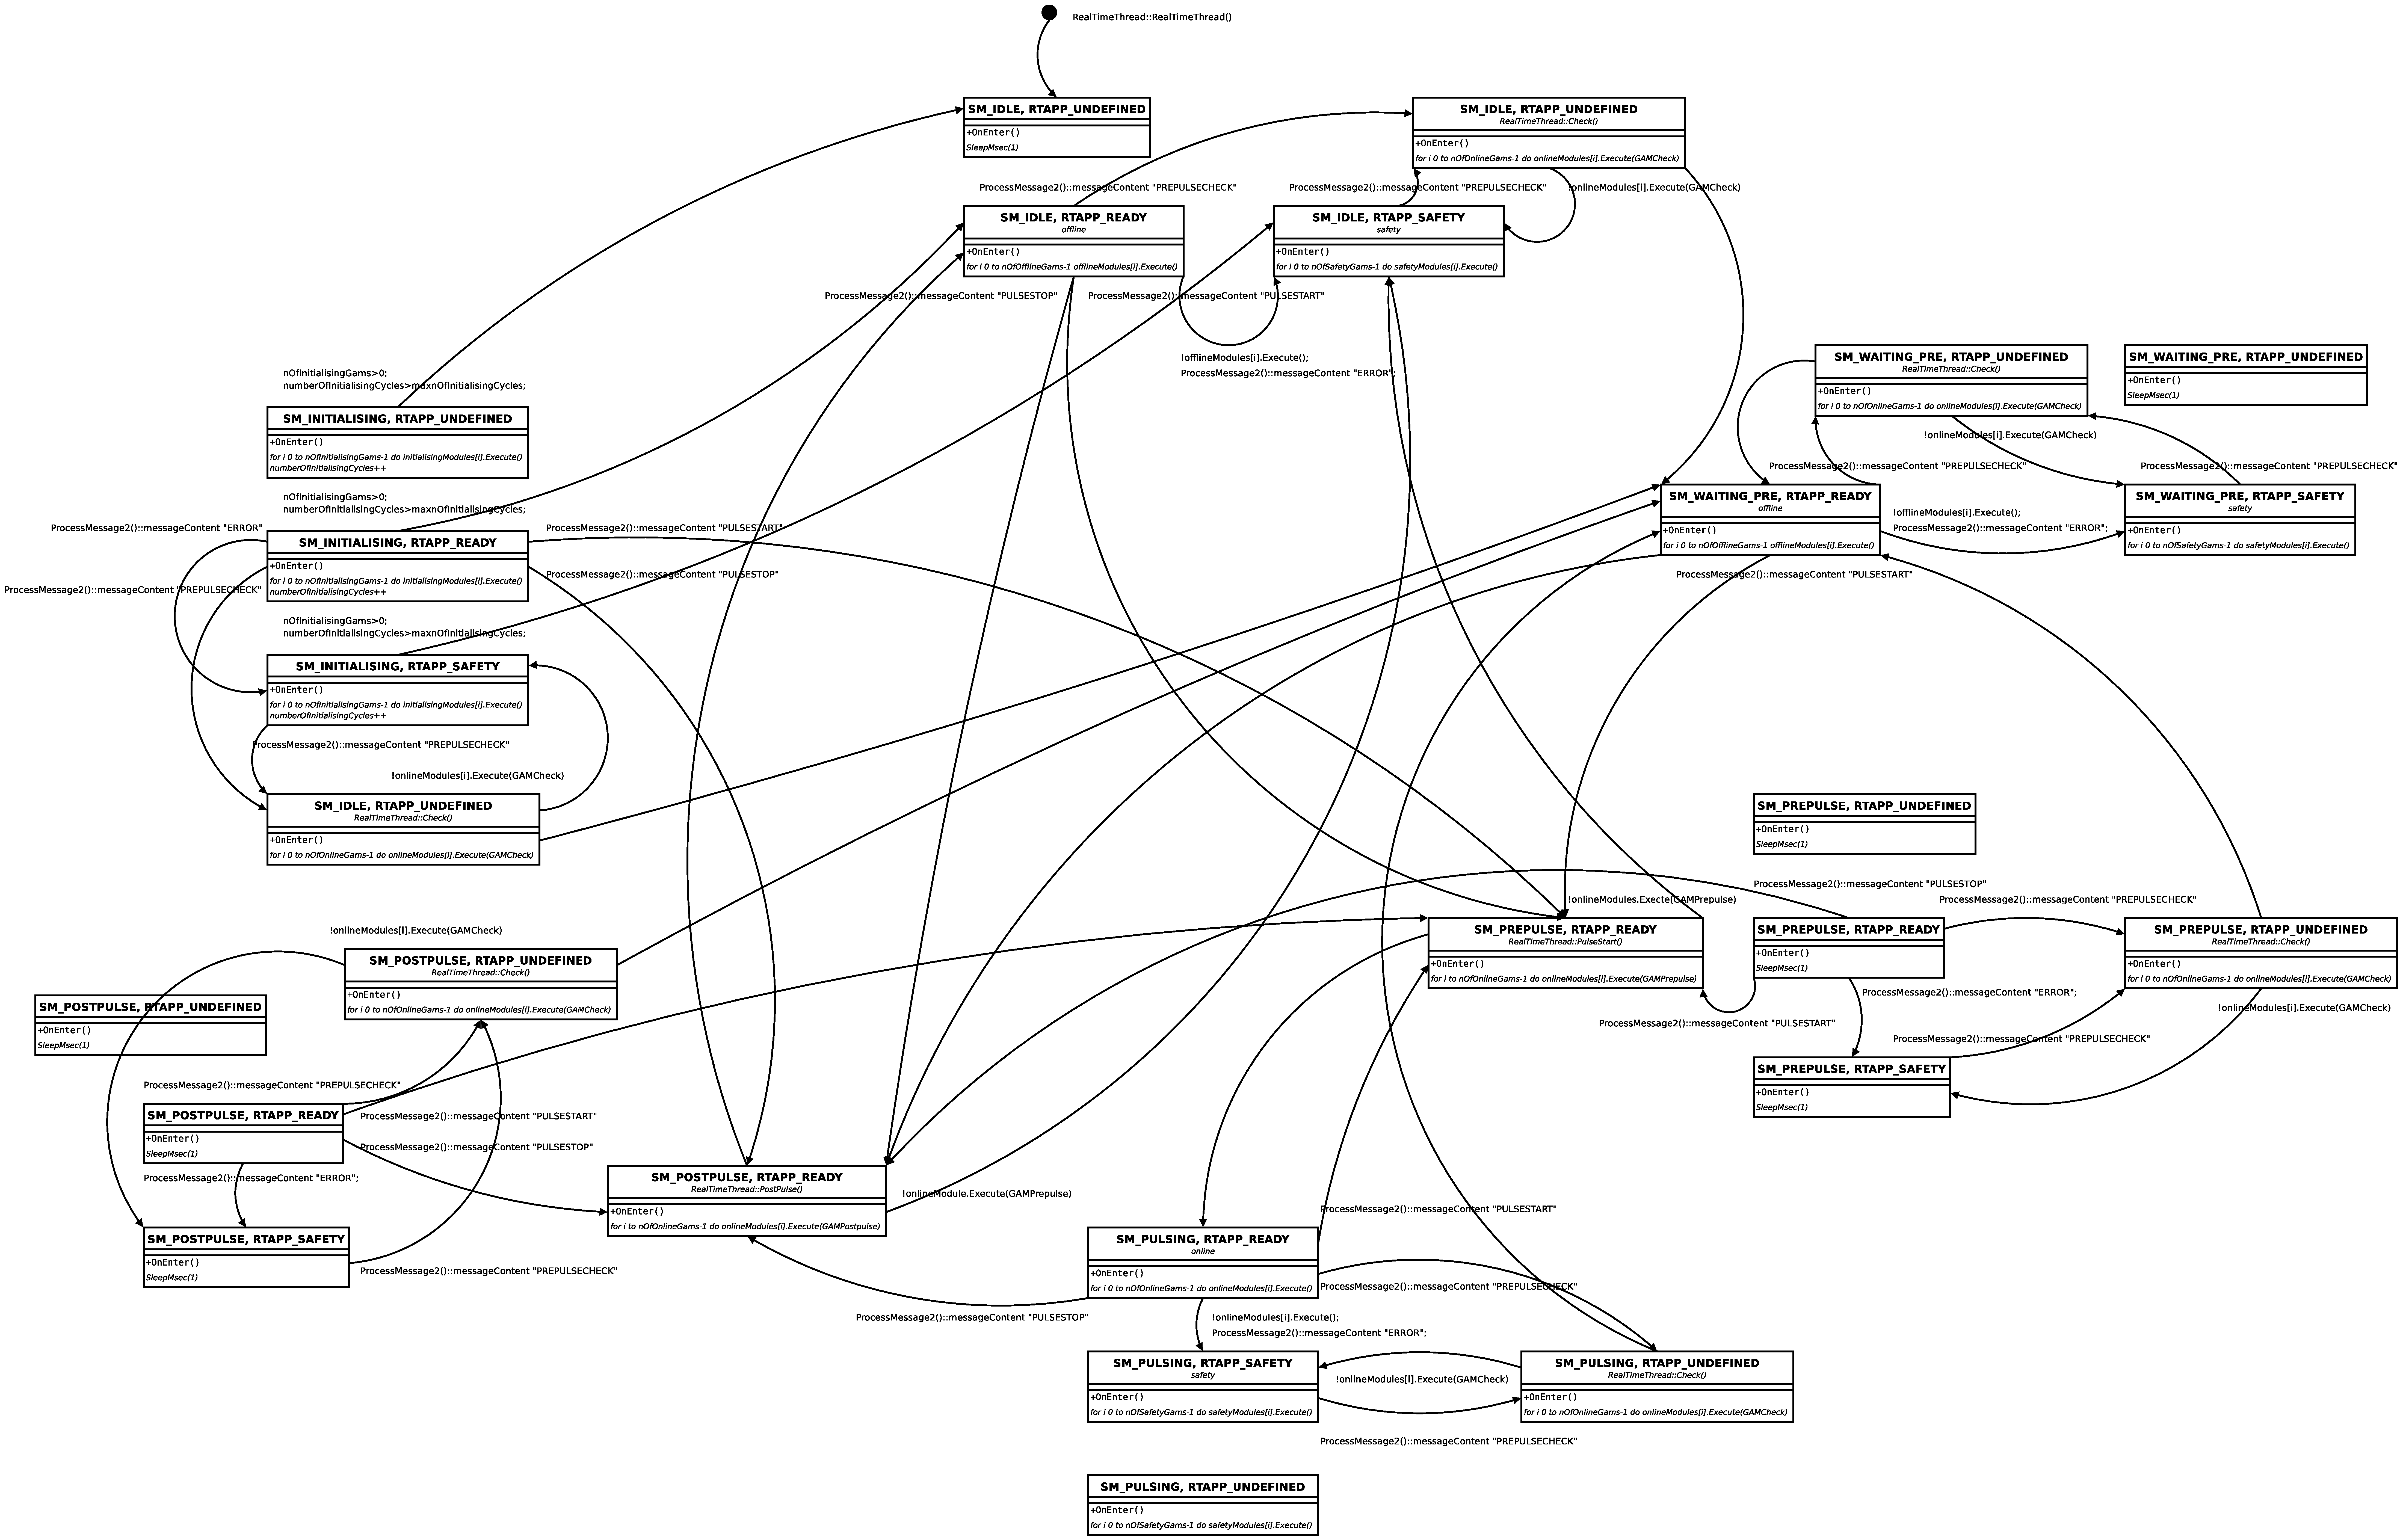
\includegraphics[width=\textwidth]{MARTe/RealTimeThreadSM.eps}
 \caption{MARTe \texttt{RealTimeThread} current internal state machine}
 \label{f:MARTe:RealTimeThread:StateMachine}
\end{sidewaysfigure}
\clearpage



Continuing with the attributes of the \texttt{RealTimeThread} class we stop on \texttt{ddb} that is the DDB used by the real-time thread during its activities, all data between GAMs are written there.

One of the users of such DDB is the performance monitor, a performance monitor is implemented thanks to an \texttt{RTCodeSTatsStruct} object and monitors the performance of the RealTimeThread and GAMs. \texttt{performanceInterface} its a pointer to saved performance of the Real Time Thread and GAMs into the DDB. \\


The attribute \texttt{runOnCPU} identifies on which CPU the \texttt{RealTimeThread} is running; \texttt{threadID} is the thread identifier in the system, \texttt{priority} is the thread priority; \texttt{isThreadRunning} specifies if the thread is running or is dead, at the end \texttt{stopThread} requests the thread termination.

\begin{lstlisting}[
extendedchars=true,%
basicstyle=\fontfamily{pcr}\fontseries{m}\selectfont\footnotesize, %
stepnumber=1,%
numberstyle=\tiny,%
keywordstyle=\footnotesize\tt ,%
language=C++]
   GCRTemplate<DDB> ddb;

   RTCodeStatsStruct performanceMonitor;
   DDBOutputInterface* performanceInterface;

   int32 runOnCPU;
   TID threadID;
   int32 priority;
   bool isThreadRunning;
   bool stopThread;
\end{lstlisting}

The method \texttt{RTThread} implements the \texttt{RealTimeThread} activities; it executes a private state machine that runs the online, offline, safety or initializing GAMs depending on the combined state of the \texttt{RealTimeThread} (\texttt{smStatus}, \texttt{rtStatus}). The method \texttt{Start} starts the thread activities and the \texttt{Stop} stops the thread activities. \\


Then follow three methods that can be implemented inside the state machine, \texttt{PulseStart} runs the GAMs prepulse activities in response to pulse in progress message; \texttt{PostPulse} runs the GAMs postpulse activities in response to pulse in termination message; \texttt{Check} runs the GAMs check activities in response to a waiting for pre message. Note that this methods are really bounded to the plant system you are working for. \\

The method \texttt{ProcessHttpMessage} implements sources reflection using the HTTP/HTML format.

The method \texttt{ProcessMessage2} convert each message to the \texttt{RealTimeThread} in a state change to the combined internal state machine (\texttt{RTThread}), not all messages are valid for a state change. \texttt{SendMessageReply} prepares a \texttt{MessageReply} to the senders when processing message.

The method \texttt{HandleLevel1Message} stops the \texttt{RealTimeThread} on a semaphore and reinitializes all GAM according to the information stored in the CDB.

Methods \texttt{ObjectLoadSetup} and \texttt{ObjectSaveSetup} initializes and saves the thread parameters and the GAMs from the configuration file.

\begin{lstlisting}[
extendedchars=true,%
basicstyle=\fontfamily{pcr}\fontseries{m}\selectfont\footnotesize, %
stepnumber=1,%
numberstyle=\tiny,%
keywordstyle=\footnotesize\tt ,%
language=C++]
   void RTThread();
   bool Start();
   bool Stop();

   bool PulseStart();
   bool PostPulse();
   bool Check();

   virtual bool ProcessHttpMessage(HttpStream& hStream);

   virtual bool ProcessMessage2(GCRTemplate<MessageEnvelope> envelope);
   bool SendMessageReply(GCRTemplate<MessageEnvelope> envelope,bool ok);

   bool HandleLevel1Message(ConfigurationDataBase& cdb);
public:
   RealTimeThread();
   virtual ~RealTimeThread();

   bool ObjectLoadSetup(ConfigurationDataBase& info,StreamInterface* err);
   bool ObjectSaveSetup(ConfigurationDataBase& info,StreamInterface* err);
\end{lstlisting}



\subsection{MARTeMenu}
\texttt{[MARTeMenu.h, MARTeMenu.cpp]} \\
The class \texttt{MARTeMenu} follow with all its interface, it is only a specialization of the \texttt{MenuContainer} class to explicitly create a MARTe menu.

\begin{lstlisting}[
extendedchars=true,%
basicstyle=\fontfamily{pcr}\fontseries{m}\selectfont\footnotesize, %
stepnumber=1,%
numberstyle=\tiny,%
keywordstyle=\footnotesize\tt ,%
language=C++]
class MARTeMenu: public MenuContainer{
public:
   MARTeMenu();
   virtual ~MARTeMenu();

   virtual bool ObjectLoadSetup(ConfigurationDataBase& info,StreamInterface* err);
   virtual bool ObjectSaveSetup(ConfigurationDataBase& info,StreamInterface* err);
};
\end{lstlisting}



\subsection{MARTeContainer}
\texttt{[MARTeContainer.h, MARTeContainer.cpp]} \\
The class \texttt{MARTeContainer} its a container of everything you need to make a control algorithm work in real-time, i.e. its a set of threads with application blocks (GAMs) and a memory data bus, a state machine, menues, a configuration database and some error catching mechanism. Such container class inherits from \texttt{GCReferenceContainer} and \texttt{MessageHandler} it implements the \texttt{HttpInterface} interface. \\


The first attribute, \texttt{lastReceivedCDB} is a reference to the last received CDB; \texttt{sendFatalErrorMessage} adds the cabability of sending Fatal Error messages.

\texttt{stateMachineName} is the name of the \texttt{StateMachine} object associated with the current set of instantiated object (not to be confused with the internal state of a RealTimeThread); \texttt{level1Name} is the name of the CODAS Level1 handling object; \texttt{commTimeout} is the communication timeout.

The attribute \texttt{marteStaticMenu} is the static part of the menu system, \texttt{marteCommonMenu} is a reference to the general menu system. \\


The attribute \texttt{needStartStopMessage} contains all object that need a start and stop message (objects that implement the \texttt{StartStopMessageHandlerInterface}) and \texttt{realTimeThreads} contains all real-time threads (\texttt{RealTimeThread}).

\begin{lstlisting}[
extendedchars=true,%
basicstyle=\fontfamily{pcr}\fontseries{m}\selectfont\footnotesize, %
stepnumber=1,%
numberstyle=\tiny,%
keywordstyle=\footnotesize\tt ,%
language=C++]
private:
   ConfigurationDataBase lastReceivedCDB;
   GCRTemplate <MessageDeliveryRequest> sendFatalErrorMessage;
   FString stateMachineName;
   FString level1Name;
   TimeoutType commTimeout;

   GCRTemplate <MenuContainer> marteStaticMenu;
   GCRTemplate <MenuContainer> marteCommonMenu;

   GCReferenceContainer needStartStopMessage;
   GCReferenceContainer realTimeThreads;
\end{lstlisting}

The method \texttt{CreateMenuInterfaces} creates the system menus dynamically.

The method \texttt{StartAllActivities} send the start message to all object in \texttt{needStartStopMessage} attribute; \texttt{StopAllActivities} send a stop message to all object in \texttt{needStartStopMessage};  \texttt{ForwardMessageRequest} forwards a message to all object in \texttt{needStartStopMessage}. \\


The method \texttt{ProcessMessage} is the message handling routine, \texttt{ProcessHttpMessage} is the main entry point for \texttt{HttpInterface}.

\begin{lstlisting}[
extendedchars=true,%
basicstyle=\fontfamily{pcr}\fontseries{m}\selectfont\footnotesize, %
stepnumber=1,%
numberstyle=\tiny,%
keywordstyle=\footnotesize\tt ,%
language=C++]
   bool CreateMenuInterfaces();

   bool StartAllActivities();
   bool StopAllActivities();

   bool ForwardMessageRequest(GCRTemplate<MessageEnvelope> gcrtme);
   bool ProcessLevel1Message(ConfigurationDataBase& level1);

public:
   MARTeContainer();
   virtual ~MARTeContainer();

   virtual bool ProcessMessage(GCRTemplate<MessageEnvelope> envelope);
   virtual bool ProcessHttpMessage(HttpStream& hStream);

   virtual bool ObjectLoadSetup(ConfigurationDataBase& info,StreamInterface* err);
   virtual bool ObjectSaveSetup(ConfigurationDataBase& info,StreamInterface* err);
\end{lstlisting}



\subsection{Design Notes}
A more dynamic structure to handle the performance data can be created, i.e. data can grow dynamically also if allocated statically each relative sample must be near the absolute one. As everything in this project is a bit strange that there is any generic interface to plug in a sort of generic performance code measurement tool. \\


The \texttt{RealTimeThread} has two state machines that interact between them; this interaction is not well defined and some spurious state are not well managed, Figure \ref{f:MARTe:RealTimeThread:StateMachine} illustrate it; the addition of methods \texttt{Check}, \texttt{PulseStart} and \texttt{PostPulse} complicate more and more the system and should be integrated in the state machine. Another notes is that if the plant system's state machine goes wrong also the \texttt{RealTimeThread}'s state machine goes wrong, no check is done.

In any case the private state machine of the \texttt{RealTimeThread} must be rewritten for generality but also for correcteness; in general the ideaa to have two state machines one that reflect the status of the plant and one that reflect the state of the \texttt{RealTimeThread} is a good idea, the final state machine will be a combination of those states. \\


Also the \texttt{MARTeContainer} is not so generic as it would be; infact it require a \texttt{level1Name} string that associate to them a \textit{Level1} object that is a JET related entity, not to be founded in any other experiments. \\



\section{MARTe}
MARTe as we said is no more then a \texttt{MarteContainer} but not all components in MARTe are instantiated by the \texttt{MarteContainer} so we need some more code that loads for example the state machine or the level1 interface. Such code is in the following executables that are really executables and so can also be executed by the Operating System on which are loaded. The only difference between those is that \texttt{MARTe} is a normal executable running on a console and \texttt{MARTeService} is a service, it doesn't require a console to execute, both works in Microsoft Windows$^\copyright$ and UNIX like operating systems. Both executables require only one command line paramenter that is the configuration file form wich they load all required serialized components.
/** Real time manager. */


\subsubsection{MARTe}
\texttt{[MARTe.cpp]}\\
Note that \texttt{MARTe.h} is not included in \texttt{MARTe.cpp}, \texttt{MARTe.h} is to be considered old and must be deleted from the directory.

\begin{lstlisting}[
extendedchars=true,%
basicstyle=\fontfamily{pcr}\fontseries{m}\selectfont\footnotesize, %
stepnumber=1,%
numberstyle=\tiny,%
keywordstyle=\footnotesize\tt ,%
language=C++]
static bool initialized;
static EventSem sem;

int main(int argc, char* argv[]);
int InitGlobalContainer(const void* fileName);
int StartMARTeActivities();
int StopMARTeActivities();
int MARTeMenu();
\end{lstlisting}



\subsubsection{MARTeService}
\texttt{[MARTeService.h, MARTeService.cpp]}\\

\begin{lstlisting}[
extendedchars=true,%
basicstyle=\fontfamily{pcr}\fontseries{m}\selectfont\footnotesize, %
stepnumber=1,%
numberstyle=\tiny,%
keywordstyle=\footnotesize\tt ,%
language=C++]
class MARTeService: public WindowsServiceApplication {
   ConfigurationDataBase cdb;

private:
   virtual bool ServiceInit();
   virtual bool ServiceStart();
   virtual bool ServiceStop();

public:
   MARTeService(const char *serviceName,const char *title):
      WindowsServiceApplication(serviceName,title){
    }
};
\end{lstlisting}



\section{Design Notes}
There are some clean up to do in the main directory of MARTe and also in \textit{MarteSupportLib} directory.

In the main directory would be likely to remove the \textit{MARTeTrainer.cpp} and the \texttt{text.cpp} applications used to test the whole system. The file \texttt{RealTimeThreadPool.h} is also to be considered old stuff and must be deleted, the thread's pool is now integrated in the \texttt{MarteContainer}, also \texttt{MARTe.h} must deleted. For the same reasons the \texttt{MObject}s and the \texttt{MObjectPool} are not existents right now and the code of \texttt{MARTe.h} must be cleaned up.

In the directory \textit{MarteSupportLib} all the \textbf{MPIC} stuff must be moved.


